% =============================================================================
%  Soutenance de stage : Parler aux avions
%  Nicolas Marano - M1 Calcul Haute Performance, Simulation (HPC, Image, IA)
%  Compilation : pdflatex x2 (voir presentation/build.sh)
% =============================================================================
\documentclass[aspectratio=169,11pt]{beamer}

\usetheme[progressbar=frametitle, numbering=fraction, block=fill]{metropolis}

\usepackage[utf8]{inputenc}
\usepackage[T1]{fontenc}
\usepackage[french]{babel}
\usepackage[sfdefault]{FiraSans}
\usepackage{FiraMono}
\usepackage{graphicx}
\usepackage{booktabs}
\usepackage{array}
\usepackage{xcolor}
\usepackage{tikz}
\usepackage{adjustbox}
\usepackage{appendixnumberbeamer}
\usetikzlibrary{positioning, arrows.meta, shapes.geometric, fit, calc,
                decorations.pathreplacing, shapes.symbols, backgrounds}

% ---------------------------------------------------------------- palette ---
\definecolor{bleu}{HTML}{1F4E79}
\definecolor{ambre}{HTML}{B26B00}
\definecolor{ardoise}{HTML}{475569}
\definecolor{vert}{HTML}{15803D}
\definecolor{rouge}{HTML}{B4232A}
\definecolor{clair}{HTML}{F1F5F9}
\definecolor{nuit}{HTML}{0E1726}

\setbeamercolor{frametitle}{bg=bleu, fg=white}
\setbeamercolor{progress bar}{fg=ambre, bg=bleu!25}
\setbeamercolor{alerted text}{fg=ambre}
\setbeamercolor{normal text}{fg=ardoise!95, bg=white}
\setbeamercolor{title separator}{fg=ambre}
\setbeamercolor{section title}{fg=bleu}
\setbeamercolor{block title}{bg=bleu!12, fg=bleu}
\setbeamercolor{palette primary}{bg=bleu, fg=white}
\setbeamercolor{block body}{bg=bleu!4}
\setbeamerfont{frametitle}{size=\large}
\setbeamertemplate{itemize items}{\color{ambre}\textbullet}
\metroset{block=fill}

% ------------------------------------------------------------------ outils ---
% carte de metrique : gros chiffre + legende
\newcommand{\metric}[3][ambre]{%
  \begin{tikzpicture}[baseline]
    \node[rounded corners=4pt, draw=#1!55, fill=#1!7, line width=0.7pt,
          inner sep=9pt, minimum width=4.3cm, align=center]
      {\fontsize{27}{30}\selectfont\bfseries\color{#1}#2\\[4pt]
       \normalfont\scriptsize\color{ardoise}#3};
  \end{tikzpicture}}

% carte de metrique compacte
\newcommand{\metricsm}[3][ardoise]{%
  \begin{tikzpicture}[baseline]
    \node[rounded corners=3pt, draw=#1!45, fill=#1!5, line width=0.6pt,
          inner sep=6pt, minimum width=3.2cm, align=center]
      {\fontsize{17}{19}\selectfont\bfseries\color{#1}#2\\[3pt]
       \normalfont\tiny\color{ardoise}#3};
  \end{tikzpicture}}

% mention de source, en pied de slide
\newcommand{\src}[1]{\vfill{\tiny\color{ardoise!70}#1}}

% phrase-cle detachee
\newcommand{\cle}[1]{{\large\color{bleu}\textbf{#1}}}

% fond image plein cadre + voile sombre
\newcommand{\bgimage}[2]{%
  \usebackgroundtemplate{%
    \begin{tikzpicture}[remember picture, overlay]
      \node[inner sep=0pt] at (current page.center)
        {\includegraphics[height=\paperheight]{#1}};
      \fill[nuit, opacity=#2] (current page.south west)
        rectangle (current page.north east);
    \end{tikzpicture}}}
\newcommand{\bgclear}{\usebackgroundtemplate{}}
% aplat de couleur plein cadre (un fond vide masquerait la couleur de canvas)
\newcommand{\bgfill}[1]{%
  \usebackgroundtemplate{%
    \begin{tikzpicture}[remember picture, overlay]
      \fill[#1] (current page.south west)
        rectangle (current page.north east);
    \end{tikzpicture}}}

% styles TikZ communs
\tikzset{
  bloc/.style   = {rounded corners=3pt, draw=ardoise!55, fill=white, line width=0.7pt,
                   align=center, font=\scriptsize, text=ardoise, inner sep=4pt},
  blocia/.style = {bloc, dashed, draw=ardoise!70, fill=ardoise!4},
  bloccode/.style={bloc, draw=ambre, fill=ambre!12, text=ambre!75!black, line width=1pt},
  fl/.style     = {-{Stealth[length=2.4mm]}, ardoise!65, line width=0.9pt},
  flg/.style    = {-{Stealth[length=2.4mm]}, vert, line width=1.1pt},
  flr/.style    = {-{Stealth[length=2.4mm]}, rouge, line width=1.1pt},
  etiq/.style   = {font=\tiny, text=ardoise!85, align=center},
}

% ------------------------------------------------------------------ titre ---
\title{Parler aux avions}
\subtitle{Un simulateur d'entraînement au contrôle aérien piloté par la voix}
\author{Nicolas Marano}
\institute{M1 Calcul Haute Performance, Simulation (HPC, Image, IA)\\
Laboratoire LICIIS, URCA \enskip$\cdot$\enskip Calcul : supercalculateur ROMEO}
\date{Soutenance de stage \enskip$\cdot$\enskip 2026}

% =============================================================================
\begin{document}

% --- 1. Titre, plein cadre sombre ------------------------------------------
\bgimage{figures/app_radar.png}{0.60}
\begin{frame}[plain]
  \vfill
  \begin{minipage}{0.68\textwidth}
  {\color{white}\fontsize{32}{36}\selectfont\bfseries Parler aux avions\par}
  \vspace{4pt}
  \textcolor{ambre}{\rule{45mm}{1.6pt}}\\[10pt]
  {\color{white!85}\normalsize Un simulateur d'entraînement au contrôle
   aérien piloté par la voix\par}
  \vspace{14pt}
  {\color{white!70}\footnotesize
   Nicolas Marano \enskip$\cdot$\enskip M1 HPC \& Simulation, URCA\\[2pt]
   Laboratoire LICIIS \enskip$\cdot$\enskip Calcul : supercalculateur
   ROMEO (GH200)\par}
  \end{minipage}
  \vspace{8pt}
\end{frame}
\bgclear

\note{Bonjour. Ce que vous voyez derriere le titre n'est pas une maquette :
c'est l'application qui tourne. Le sujet de ce stage n'est ni un modele d'IA
ni un simulateur de trafic, c'est un dialogue radio.}

% --- 2. Le verrou -----------------------------------------------------------
\begin{frame}{L'élève parle, personne ne répond}
\centering
\begin{tikzpicture}[scale=0.86, transform shape]

  % ---- panneau gauche : aujourd'hui
  \node[etiq, font=\scriptsize\bfseries, text=ardoise] at (-3.6,3.0) {AUJOURD'HUI};
  \node[bloc, minimum width=1.9cm, minimum height=1.0cm] (eleve) at (-5.6,1.4)
       {élève\\contrôleur};
  \node[bloc, minimum width=1.9cm, minimum height=1.0cm, fill=ardoise!10] (instr) at (-1.7,1.4)
       {instructeur\\\emph{pseudo-pilote}};
  \node[etiq, text=ambre!80!black, font=\tiny\itshape] (parole) at (-3.65,2.15)
       {« Air France 300, descendez niveau 180 »};
  \draw[fl, ambre] (eleve.east) -- (instr.west);

  \draw[ardoise!35, line width=0.5pt] (instr.south) -- (-1.7,-1.85);
  \foreach \i/\c in {0/AFR1234, 1/BAW57, 2/DLH88, 3/RYR9, 4/EZY41, 5/SAS22}{
    \node[etiq, font=\tiny, text=ardoise!70, fill=white, inner sep=1.3pt]
         at (-1.7,{0.35-\i*0.42}) {\c};
  }
  \node[etiq, text=ardoise, font=\scriptsize] at (-3.6,-2.35)
       {un opérateur mobilisé\\pour un seul élève};

  % ---- separateur
  \draw[ardoise!30, line width=0.6pt] (0.35,-2.9) -- (0.35,3.2);

  % ---- panneau droit : objectif
  \node[etiq, font=\scriptsize\bfseries, text=bleu] at (4.3,3.0) {OBJECTIF};
  \node[bloc, minimum width=1.9cm, minimum height=1.0cm] (eleve2) at (2.3,1.4)
       {élève\\contrôleur};
  \node[bloccode, minimum width=2.1cm, minimum height=1.0cm, dashed] (ia) at (6.3,1.4)
       {\textbf{?}};
  \node[etiq, text=ambre!80!black, font=\tiny\itshape] at (4.3,2.15)
       {« Air France 300, descendez niveau 180 »};
  \draw[fl, ambre] (eleve2.east) -- (ia.west);
  \draw[fl, bleu] ([yshift=-3pt]ia.west) to[out=200, in=340]
        node[etiq, below, pos=0.5, text=bleu]{réponse} ([yshift=-9pt]eleve2.east);

  \draw[ardoise!35, line width=0.5pt] (ia.south) -- (6.3,-1.85);
  \foreach \i/\c in {0/AFR1234, 1/BAW57, 2/DLH88, 3/RYR9, 4/EZY41, 5/SAS22}{
    \node[etiq, font=\tiny, text=ardoise!70, fill=white, inner sep=1.3pt]
         at (6.3,{0.35-\i*0.42}) {\c};
  }
  \node[etiq, text=bleu, font=\scriptsize] at (4.3,-2.35)
       {les avions répondent\\sans opérateur};
\end{tikzpicture}

\vspace{2pt}
{\small La radio est le geste central du métier. C'est aussi le plus cher à
répéter.}
\end{frame}

\note{Le verrou pedagogique n'est ni le radar ni la physique de vol : c'est
l'absence d'interlocuteur. Automatiser le pilote, pas le radar.}

% --- 3. La boucle en cinq boites -------------------------------------------
\begin{frame}{La boucle radio, en cinq étapes}
\centering
\begin{tikzpicture}[scale=0.88, transform shape]
  \def\dx{2.85}
  \node[blocia, minimum width=2.3cm, minimum height=1.35cm] (b1) at (0,0)
       {\textbf{ENTENDRE}\\la parole\\devient du texte};
  \node[blocia, minimum width=2.3cm, minimum height=1.35cm] (b2) at (\dx,0)
       {\textbf{COMPRENDRE}\\le texte devient\\un ordre};
  \node[bloccode, minimum width=2.3cm, minimum height=1.7cm] (b3) at (2*\dx,0)
       {\textbf{VÉRIFIER}\\le code accepte\\ou refuse};
  \node[bloc, minimum width=2.3cm, minimum height=1.35cm] (b4) at (3*\dx,0)
       {\textbf{EXÉCUTER}\\l'avion\\manœuvre};
  \node[blocia, minimum width=2.3cm, minimum height=1.35cm] (b5) at (4*\dx,0)
       {\textbf{RÉPONDRE}\\collationnement\\en voix radio};

  \foreach \i/\j in {1/2, 2/3, 3/4, 4/5}{\draw[fl] (b\i) -- (b\j);}

  % outils + temps mesures
  \node[etiq, below=3pt of b1] {Whisper adapté\\\textbf{0,36 s}};
  \node[etiq, below=3pt of b2] {LLM ancré OACI\\\textbf{1,06 s}};
  \node[etiq, below=8pt of b3, text=ambre!80!black] {validateur\\\textbf{déterministe}};
  \node[etiq, below=3pt of b4] {BlueSky\\\textbf{$<$ 0,01 s}};
  \node[etiq, below=3pt of b5] {synthèse + VHF\\\textbf{1,15 s}};

  % pastilles nature
  \node[etiq, above=2pt of b1, text=ardoise!70] {modèle};
  \node[etiq, above=2pt of b2, text=ardoise!70] {modèle};
  \node[etiq, above=5pt of b3, text=ambre, font=\tiny\bfseries] {CODE TESTÉ};
  \node[etiq, above=2pt of b4, text=ardoise!70] {code};
  \node[etiq, above=2pt of b5, text=ardoise!70] {modèle};

  % boucle de retour
  \draw[fl, bleu] (b5.east) -- (13.0,0) -- (13.0,-2.35)
        -- node[etiq, above, text=bleu]{l'élève entend la réponse et enchaîne}
        (-2.5,-2.35) -- (-2.5,0) -- (b1.west);

  \node[rounded corners=3pt, draw=bleu!45, fill=bleu!6, inner sep=5pt,
        font=\scriptsize, text=bleu] at (2*\dx,2.35)
        {boucle complète mesurée : \textbf{2,6 s}};
\end{tikzpicture}
\src{Latences moyennes, $n = 25$ clairances parlées \enskip$\cdot$\enskip
     \texttt{bench/results/e2e\_bench.json}}
\end{frame}

\note{Voila la carte du territoire. Cinq etages, une boucle fermee, 2,6 s.
Trois etages sont des modeles probabilistes, deux sont du code teste. Retenez
la boite ambre : c'est elle le sujet du slide suivant.}

% --- 4. Le pivot : le modele propose, le code verifie -----------------------
\begin{frame}{Le modèle propose, le code vérifie}
\centering
\begin{tikzpicture}[scale=0.80, transform shape]

  % le mur, avec son bandeau de titre integre
  \fill[ambre!14, rounded corners=4pt] (-2.4,-2.05) rectangle (2.4,2.15);
  \fill[ambre, rounded corners=4pt] (-2.4,1.42) rectangle (2.4,2.15);
  \fill[ambre] (-2.4,1.42) rectangle (2.4,1.72);
  \draw[ambre, line width=1.2pt, rounded corners=4pt] (-2.4,-2.05) rectangle (2.4,2.15);
  \node[font=\scriptsize\bfseries, text=white] at (0,1.79)
       {VALIDATION DÉTERMINISTE};

  \foreach \y/\t in {
     0.82/{niveau dans les limites de l'avion ?},
     0.02/{cap entre 0 et 360 ?},
    -0.78/{point de report connu du secteur ?},
    -1.62/{descendre \emph{vers le haut} ?}}{
    \node[rounded corners=2pt, fill=white, draw=ambre!55, line width=0.6pt,
          minimum width=4.4cm, minimum height=0.66cm, align=center,
          font=\scriptsize, text=ardoise] at (0,\y) {\t};}

  % le modele, a gauche
  \node[cloud, cloud puffs=11, cloud ignores aspect, draw=ardoise!70, dashed,
        fill=ardoise!5, minimum width=2.9cm, minimum height=1.5cm,
        align=center, font=\scriptsize, text=ardoise] (nuage) at (-5.6,0.5)
       {le modèle\\propose};
  \draw[fl] (nuage.east) -- node[etiq, above, pos=0.55]{ordre} (-2.45,0.5);

  % sortie acceptee
  \node[bloc, fill=vert!8, draw=vert!70, minimum width=2.5cm,
        minimum height=1.1cm, text=vert!60!black] (bs) at (5.4,0.5)
       {\textbf{BlueSky}\\exécute la manœuvre};
  \node[font=\scriptsize, text=vert!50!black, align=center] at (5.4,-1.35)
       {\textbf{0} ordre hors bornes\\exécuté sur 116 clairances};
  \draw[flg] (2.45,0.5) -- (bs.west);

  % refus : retour vers le modele, sous le mur
  \draw[flr] (-2.45,-1.62) -- (-5.6,-1.62) -- (nuage.south);
  \node[font=\scriptsize, text=rouge, align=center] at (-4.0,-2.05)
       {refusé : l'avion reste muet};

  % contournement impossible
  \draw[ardoise!45, dashed, line width=0.8pt]
        (nuage.north) to[out=75, in=105] (bs.north);
  \draw[rouge, line width=1.5pt] (-0.32,2.53) -- (0.32,3.17);
  \draw[rouge, line width=1.5pt] (0.32,2.53) -- (-0.32,3.17);
  \node[font=\scriptsize, text=ardoise!75] at (0,3.6)
       {aucun chemin ne contourne le mur};
\end{tikzpicture}

\vspace{4pt}
{\small Aucune sortie de modèle n'atteint le simulateur sans passer par du code
testé : \alert{810 des 1\,871 ordres proposés} ont été rejetés.\par}
\end{frame}

\note{C'est LA phrase de la soutenance. La surete ne vient pas de la qualite
du modele, elle vient de l'architecture. C'est la reponse par avance a la
question : et si l'IA se trompe ?}

% =============================================================================
\section{Ce qu'il a fallu construire}

% --- 5. Le banc d'essai -----------------------------------------------------
\bgimage{figures/app_exercice.png}{0.30}
\begin{frame}[plain]
  \vspace{4pt}
  {\color{white}\large\textbf{Pour éprouver la voix, il a fallu bâtir tout le reste}\par}
  \vfill
  \hfill
  \begin{minipage}{0.50\linewidth}
    \raggedleft\color{white!88}\scriptsize
    conflits programmés\\
    vent et cellules orageuses\\
    poste instructeur, notation en direct\\[8pt]
    {\color{ambre}\fontsize{20}{22}\selectfont\bfseries 15 ms}\\[3pt]
    {\color{white!75}\tiny pour simuler \textbf{1 seconde} de trafic
     avec 200 aéronefs\\
     à comparer aux 2,6 s de la boucle vocale : la simulation\\
     n'est jamais le facteur limitant}
  \end{minipage}
  \vspace{10pt}
\end{frame}
\bgclear

\note{Le radar, le trafic, les conflits, le debriefing : ce n'est pas le
sujet, c'est la condition d'existence de la mesure. Sans eux, aucune boucle
vocale n'est testable.}

% --- 6. Un banc par brique --------------------------------------------------
\begin{frame}{Un banc par brique, un fichier par chiffre}
\centering
\begin{tikzpicture}[scale=0.84, transform shape]
  \foreach \i/\n in {0/{reconnaissance vocale}, 1/{interprétation},
                     2/{simulation}, 3/{synthèse vocale}, 4/{boucle complète}}{
    \node[bloc, text width=3.5cm, minimum height=0.62cm] (a\i)
         at (-4.6,{1.5-\i*0.85}) {banc \n};
    \node[bloc, minimum width=2.9cm, minimum height=0.62cm, font=\tiny\ttfamily,
          fill=clair] (b\i) at (0.2,{1.5-\i*0.85}) {};
    \draw[fl] (a\i.east) -- (b\i.west);}
  \node[font=\tiny\ttfamily, text=ardoise] at (0.2,1.5)  {stt\_bench.json};
  \node[font=\tiny\ttfamily, text=ardoise] at (0.2,0.65) {llm\_bench.json};
  \node[font=\tiny\ttfamily, text=ardoise] at (0.2,-0.2) {sim\_bench.json};
  \node[font=\tiny\ttfamily, text=ardoise] at (0.2,-1.05){tts\_bench.json};
  \node[font=\tiny\ttfamily, text=ardoise] at (0.2,-1.9) {e2e\_bench.json};

  \node[bloc, minimum width=3.0cm, minimum height=0.75cm, fill=bleu!5,
        draw=bleu!45] (fig) at (4.9,1.05) {figures du rapport};
  \node[bloc, minimum width=3.0cm, minimum height=0.75cm, fill=ambre!8,
        draw=ambre!60] (sl) at (4.9,-0.35) {chiffres de cette soutenance};
  \draw[fl] (1.75,0.5) -- (fig.west);
  \draw[fl] (1.75,-0.5) -- (sl.west);

  \node[bloc, minimum width=3.4cm, minimum height=0.6cm, fill=ardoise!5,
        font=\tiny] at (0.2,-2.85)
       {\texttt{versions.json} : matériel et versions figés};
\end{tikzpicture}

\vspace{4pt}
{\small Aucun chiffre n'est saisi à la main : chacun est lu dans un fichier
de résultats versionné.}
\src{Campagne rejouée un mois plus tard : métriques identiques champ à champ.}
\end{frame}

\note{Protocoles seedes, resultats versionnes, campagne rejouable. C'est ce
qui distingue une demonstration d'une demo.}

% =============================================================================
% --- 6bis. Emprunte / ecrit --------------------------------------------------
\begin{frame}{Ce que j'ai emprunté, ce que j'ai écrit}
\centering
\begin{tikzpicture}[scale=0.82, transform shape,
  col/.style={rounded corners=3pt, line width=0.8pt, text width=5.9cm,
              align=left, font=\scriptsize, inner sep=8pt, anchor=north}]

  \node[etiq, font=\scriptsize\bfseries, text=ardoise] at (-3.5,2.95)
       {LA COMMUNAUTÉ};
  \node[col, draw=ardoise!45, fill=ardoise!5, text=ardoise] at (-3.5,2.5)
       {\textbf{Calcul} \\ supercalculateur ROMEO, n\oe ud GH200\\[3pt]
        \textbf{Corpus} \\ ATCO2, UWB-ATCC, ATCOSIM\\
        {\tiny 3 corpus de radio réelle, transcrits par d'autres}\\[3pt]
        \textbf{Modèles} \\ Whisper, Mistral, Qwen, XTTS, Kokoro\\[3pt]
        \textbf{Simulateur} \\ BlueSky et ses modèles de performances};

  \draw[ardoise!30, line width=0.6pt] (0.15,-2.75) -- (0.15,3.15);

  \node[etiq, font=\scriptsize\bfseries, text=ambre!80!black] at (3.8,2.95)
       {CE STAGE};
  \node[col, draw=ambre!65, fill=ambre!8, text=ambre!75!black] at (3.8,2.5)
       {le canal radio VHF simulé\\[2pt]
        le graphe de secteur \emph{et} son validateur\\[2pt]
        les 9 fiches de phraséologie\\[2pt]
        \textbf{l'adaptateur de 14 Mo}\\[2pt]
        \textbf{la couche de validation déterministe}\\[2pt]
        le moteur d'exercices et son barème\\[2pt]
        l'application d'entraînement\\[2pt]
        le banc de mesure et ses corpus annotés};
\end{tikzpicture}

\vspace{4pt}
{\small Les briques d'IA viennent de la communauté. Je les ai choisies,
assemblées, adaptées et surtout \alert{mesurées}.\\
L'architecture de sûreté et l'appareil de preuve sont le travail du stage.}
\src{Inventaire complet et versions : rapport \S3.5 et \texttt{bench/results/versions.json}}
\end{frame}

\note{Diapositive de probite, et c'est la reponse a la question << qu'avez-vous
fait, vous ? >>. Ne pas s'excuser d'avoir emprunte : personne n'entraine un
modele de reconnaissance vocale depuis zero en dix semaines. Insister sur la
colonne de droite, et surtout sur les deux lignes en gras : l'adaptateur, seul
artefact de modele qui soit de moi, et la couche de validation, qui est
l'argument central du stage.}

\section{Entendre}

% --- 7. Le WER explique -----------------------------------------------------
\begin{frame}{La machine n'entend pas la radio comme nous}
\centering
\begin{tikzpicture}[scale=0.74, transform shape]
  \node[font=\scriptsize\ttfamily, text=ardoise, align=center] (ref) at (0,2.5)
       {ALFA DELTA HOLDING POINT ZERO FOUR \ EURO TRANS ONE THREE JULIETT};
  \node[etiq, above=1pt of ref, text=ardoise!70] {ce que le pilote a dit};

  \node[bloc, minimum width=11.5cm, minimum height=0.85cm, fill=rouge!4,
        draw=rouge!45, font=\scriptsize\ttfamily, text=rouge!70!black] (a) at (0,1.1)
       {ALPHA DELTA HOLDING POINT \textbf{04} \ \textbf{YOU ARE TRANSFORMED
        REDREW IT}};
  \node[etiq, left=2pt of a, anchor=east, text=ardoise] {modèle\\généraliste};

  \node[bloc, minimum width=11.5cm, minimum height=0.85cm, fill=vert!4,
        draw=vert!45, font=\scriptsize\ttfamily, text=vert!55!black] (b) at (0,-0.2)
       {ALFA DELTA HOLDING POINT ZERO FOUR \ EURO TRANS ONE THREE JULIETT};
  \node[etiq, left=2pt of b, anchor=east, text=ardoise] {modèle adapté\\au métier};

  \node[rounded corners=3pt, draw=ardoise!35, fill=clair, inner sep=6pt,
        font=\tiny, text=ardoise, align=center] at (0,-1.5)
       {taux d'erreur mots \ = \ (mots faux \ + \ mots manquants \ +
        \ mots inventés) \ $\div$ \ mots attendus};
\end{tikzpicture}

\vspace{6pt}
\metric{71,9 \% $\rightarrow$ 28,5 \%}{radio réelle ATCO2}
\hspace{14pt}
\metricsm[bleu]{91,9 \% $\rightarrow$ 19,2 \%}{corpus UWB-ATCC}
\src{Extrait réel du corpus ATCO2, condition de production (filtre VHF) :
     l'indicatif \emph{Eurotrans one three Juliett} devient
     \emph{you are transformed redrew it}
     \enskip$\cdot$\enskip \texttt{bench/results/stt\_bench.json}}
\end{frame}

\note{Definition en toutes lettres, sans symboles. Sept mots sur dix faux,
puis moins de trois. L'exemple est reel (stt_bench.json) mais c'est un cas
favorable : le modele adapte le transcrit parfaitement. Si on demande, dire
que sur les quatre autres exemples du meme fichier il reste des erreurs, et
que c'est justement pourquoi je publie un WER moyen de 28,5 % et non un
exemple. Anticiper aussi : un WER peut depasser 100 % parce que les
insertions comptent.}

% --- 8. LoRA ----------------------------------------------------------------
\begin{frame}{Adapter un modèle sans le réentraîner}
\centering
\begin{tikzpicture}[scale=0.86, transform shape]
  % le modele gele
  \node[rounded corners=4pt, fill=ardoise!12, draw=ardoise!45, line width=0.8pt,
        minimum width=9.6cm, minimum height=2.5cm, align=center,
        font=\small, text=ardoise] (base) at (0,0)
       {modèle de reconnaissance vocale\\
        \textbf{244 millions de paramètres} \enskip$\cdot$\enskip \textsc{gelé}};

  % l'adaptateur
  \node[rounded corners=2pt, fill=ambre!25, draw=ambre, line width=0.9pt,
        minimum width=0.55cm, minimum height=0.55cm] (lora) at (5.35,0) {};
  \node[etiq, right=3pt of lora, anchor=west, text=ambre!75!black, align=left]
       {adaptateur\\\textbf{14 Mo}\\$\approx$ 1,5 \% des paramètres};

  \draw[fl] (-7.2,0) -- node[etiq, above]{audio radio\\réel annoté} (base.west);
  \draw[fl] (7.55,0) -- ++(0.5,0) node[etiq, above, pos=0.5]{texte};

  \node[etiq, below=6pt of base, text=ardoise]
       {entraîné sur ATCO2 \enskip$\cdot$\enskip UWB-ATCC
        \enskip$\cdot$\enskip ATCOSIM};
\end{tikzpicture}

\vspace{10pt}
{\small On ne réécrit pas le dictionnaire : on ajoute le lexique du métier.}

\vspace{4pt}
{\footnotesize\color{rouge!80!black} Contrainte du cluster : 20 Go par
partition $\rightarrow$ un réapprentissage complet était impossible.}
\src{L'adaptateur est versionné avec le code : \texttt{model/whisper-lora-adapter}}
\end{frame}

\note{LoRA sans jargon : on gele le gros modele, on entraine 1,5 %. Et ce
choix n'est pas une mode, il est impose par les moyens reels : quota disque
de 20 Go, 8 Go de VRAM.}

% --- 9. Resultat STT --------------------------------------------------------
\begin{frame}{Deux corpus de radio réelle, une même conclusion}
\centering
\vspace{4pt}
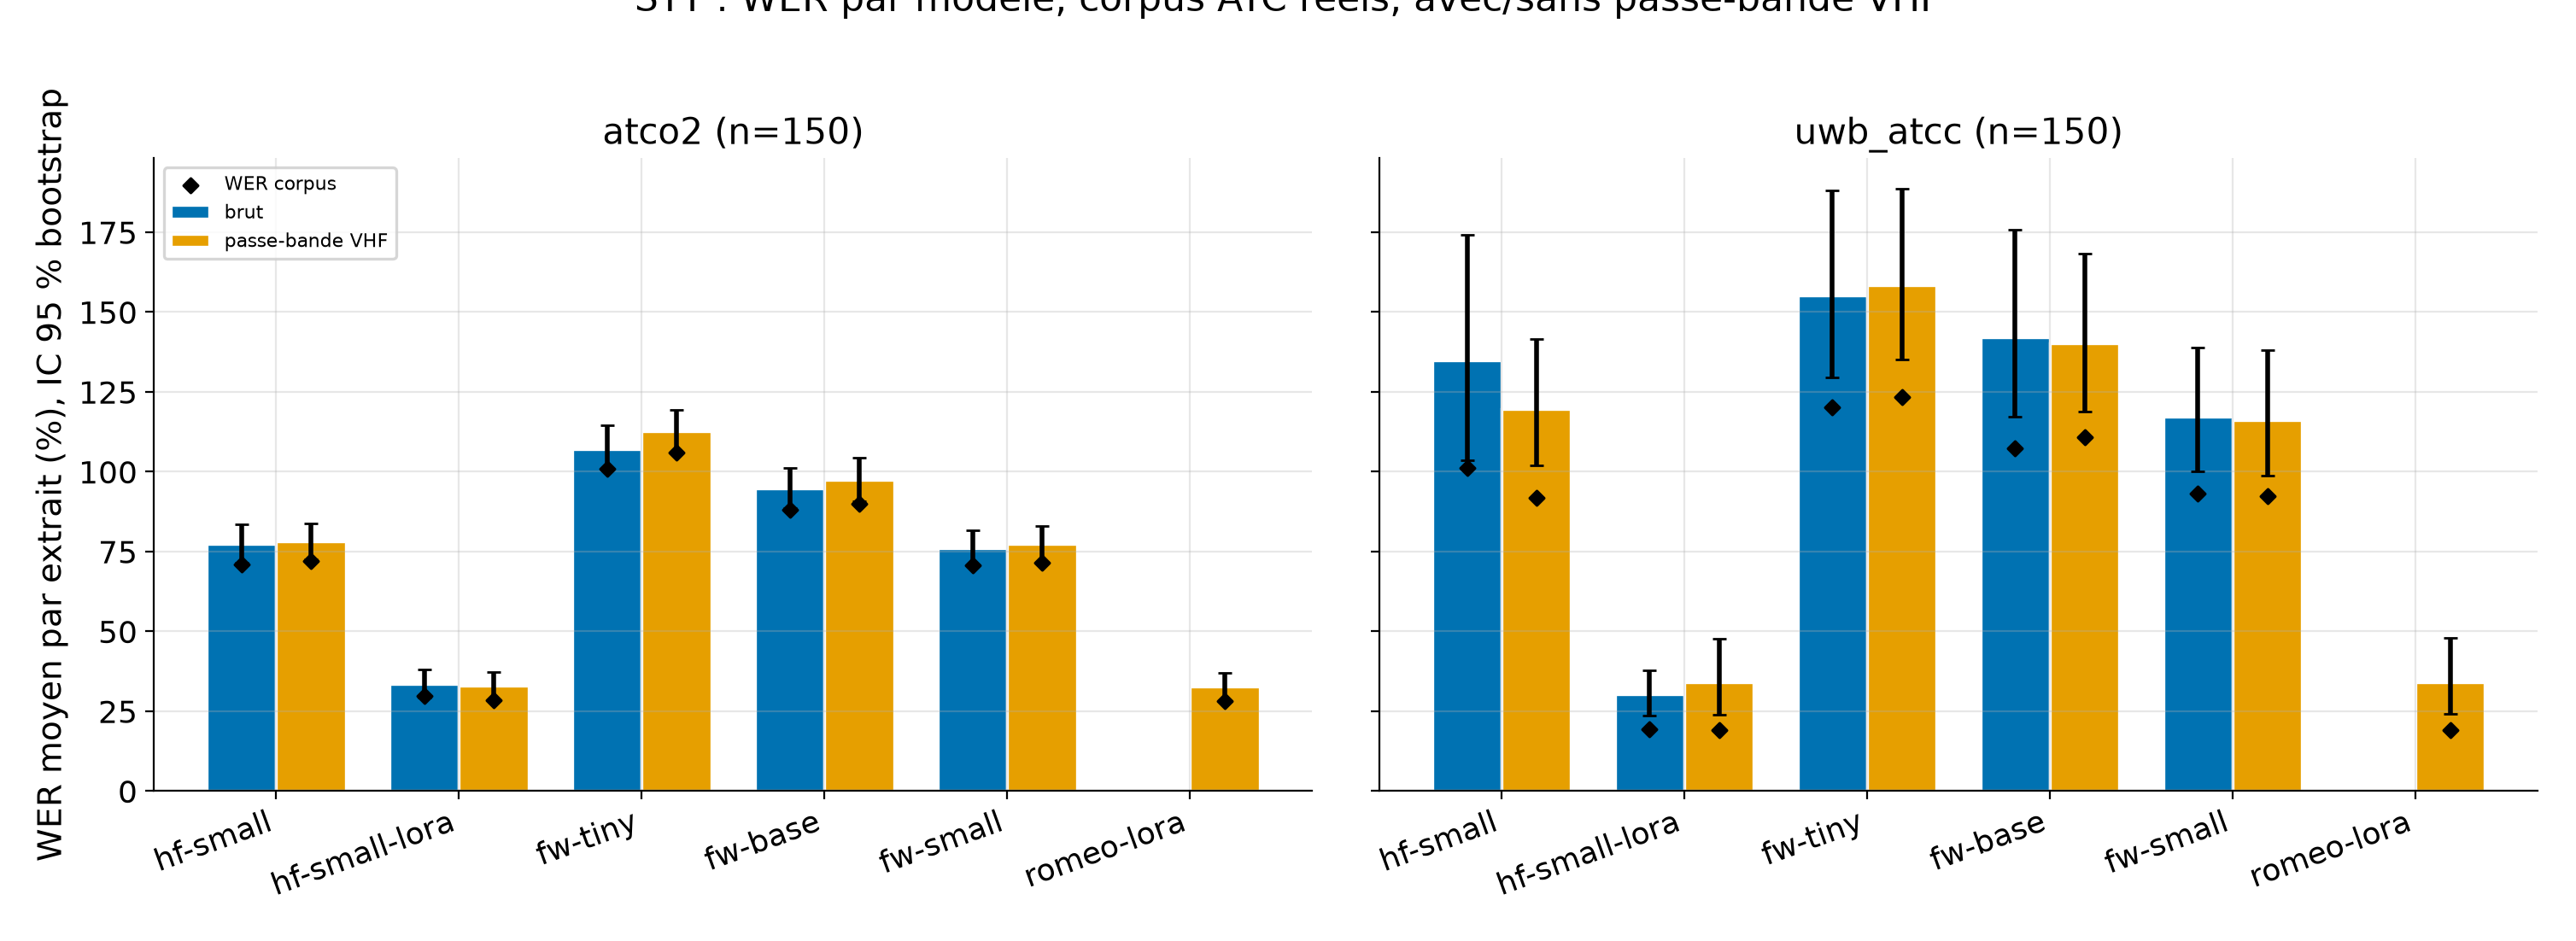
\includegraphics[width=0.92\linewidth, height=0.56\textheight, keepaspectratio]{figures/fig_stt_wer.png}

\vspace{2pt}
{\footnotesize Gain apparié sur ATCO2 : \textbf{$-45$ points}
 (IC 95 \% $[-51 ; -40]$) : l'intervalle ne touche jamais
 zéro, ce n'est pas un effet du hasard.}
\src{Les deux corpus ne se moyennent pas : accents, qualité audio et
     annotations diffèrent. \texttt{bench/results/stt\_bench.json}}
\end{frame}

\note{Le gain est mesure sur deux corpus de radio authentique et confirme
par un test statistique apparie, phrase par phrase.}

% =============================================================================
\section{Comprendre}

% --- 10. L'ancrage ----------------------------------------------------------
\begin{frame}{On ne lui demande pas de savoir : on lui met le manuel sous les yeux}
\centering
\begin{tikzpicture}[scale=0.92, transform shape]

  % (1) modele seul
  \node[etiq, font=\scriptsize\bfseries, text=ardoise] at (-5.0,2.6) {MODÈLE SEUL};
  \node[bloc, minimum width=2.6cm, minimum height=1.1cm] (m1) at (-5.0,1.2)
       {modèle de\\langage};
  \node[bloc, minimum width=3.2cm, minimum height=1.0cm, fill=rouge!5,
        draw=rouge!45, text=rouge!70!black, font=\tiny] (o1) at (-5.0,-0.6)
       {« direct GOLF ALPHA »\\$\rightarrow$ point inexistant};
  \draw[fl] (m1) -- (o1);
  \node[font=\scriptsize, text=ardoise!70, below=3pt of o1]
       {improvise avec assurance};

  % (2) modele ancre
  \node[etiq, font=\scriptsize\bfseries, text=bleu] at (0.3,2.6) {MODÈLE ANCRÉ};
  \node[bloc, minimum width=2.6cm, minimum height=1.1cm] (m2) at (0.3,1.2)
       {modèle de\\langage};
  \node[bloc, minimum width=2.4cm, minimum height=0.75cm, fill=ambre!12,
        draw=ambre!70, text=ambre!75!black, font=\tiny] (kb) at (-1.9,-0.5)
       {phraséologie\\OACI};
  \node[bloc, minimum width=2.4cm, minimum height=0.75cm, fill=ambre!12,
        draw=ambre!70, text=ambre!75!black, font=\tiny] (gr) at (2.5,-0.5)
       {graphe du\\secteur};
  \draw[fl, ambre] (kb.north) -- (m2.south west);
  \draw[fl, ambre] (gr.north) -- (m2.south east);
  \node[font=\scriptsize, text=ardoise!70] at (0.3,-1.5)
       {les documents sont fournis à chaque requête};

  % (3) sortie
  \node[etiq, font=\scriptsize\bfseries, text=ardoise] at (5.9,2.6) {SORTIE};
  \node[rounded corners=3pt, draw=ardoise!50, fill=white, line width=0.7pt,
        minimum width=3.4cm, minimum height=2.0cm, align=left,
        font=\scriptsize, text=ardoise, inner sep=6pt] (form) at (5.9,0.9)
       {indicatif \ : \ \texttt{AFR1234}\\[2pt]
        ordre \ \ \ \ \ : \ \texttt{descendre}\\[2pt]
        paramètre : \ \texttt{niveau 180}};
  \draw[fl] (m2.east) -- (form.west);
  \node[font=\scriptsize, text=ardoise!70, below=3pt of form]
       {un bordereau, pas une phrase};
\end{tikzpicture}

\vspace{2pt}
{\small Le modèle ne récite pas sa mémoire : il lit des documents qu'on lui
fournit. C'est ce qui rend sa sortie vérifiable.}
\end{frame}

\note{Demystifier l'ancrage documentaire. Le modele n'apprend pas la
phraseologie, il la consulte. Neuf fiches redigees pour le projet, plus le
graphe du secteur.}

% --- 11. Une donnee, deux usages --------------------------------------------
\begin{frame}{La même donnée informe le modèle... et le contredit}
\centering
\begin{minipage}{0.21\linewidth}
  \raggedleft\scriptsize\color{ardoise}
  \textbf{contexte donné au modèle}\\[2pt]
  les points qui existent\\vraiment dans le secteur\\[4pt]
  \textcolor{ardoise!50}{$\longrightarrow$}
\end{minipage}
\begin{minipage}{0.55\linewidth}
  \centering
  \begin{tikzpicture}[scale=0.86, transform shape,
    pt/.style={rounded corners=2pt, draw, line width=0.9pt,
               font=\tiny\bfseries, inner sep=2.6pt, align=center},
    entree/.style={pt, draw=vert!70, fill=vert!12, text=vert!45!black},
    fixe/.style={pt, draw=bleu!70, fill=bleu!12, text=bleu},
    sortie/.style={pt, draw=rouge!70, fill=rouge!10, text=rouge!75!black},
    seg/.style={ardoise!55, line width=1pt}]
    \node[entree] (ew) at (-3.5,0)  {ENTRY\_W};
    \node[fixe]   (ba) at (-1.75,0) {BALMO};
    \node[fixe]   (cr) at (0,0)     {CROSS};
    \node[fixe]   (de) at (1.75,0)  {DELTA};
    \node[sortie] (ee) at (3.5,0)   {EXIT\_E};
    \node[sortie] (no) at (0,1.5)   {NORTH};
    \node[entree] (es) at (0,-1.5)  {ENTRY\_S};
    \draw[seg] (ew) -- (ba);  \draw[seg] (ba) -- (cr);
    \draw[seg] (cr) -- (de);  \draw[seg] (de) -- (ee);
    \draw[seg] (cr) -- (no);  \draw[seg] (cr) -- (es);
    \node[font=\tiny, text=ardoise!80, align=center] at (0,-2.35)
         {7 points, 6 segments\\séparation imposée : 5 NM};
  \end{tikzpicture}
\end{minipage}
\begin{minipage}{0.21\linewidth}
  \raggedright\scriptsize\color{ambre!75!black}
  \textcolor{ambre!60}{$\longrightarrow$}\\[4pt]
  \textbf{validateur}\\[2pt]
  un point absent du graphe\\ = ordre refusé
\end{minipage}

\vspace{10pt}
{\small Le graphe du secteur sert deux fois : il renseigne le modèle, puis il
sert à le contredire.}
\end{frame}

\note{L'ancrage n'est pas seulement un contexte : c'est la meme structure de
donnees qui refuse ensuite un point de report inexistant.}

% --- 12. Le resultat qui derange --------------------------------------------
\begin{frame}{Le résultat qui dérange}
\centering
\vspace{4pt}
\metric[ardoise]{87,9 \%}{module à base de \textbf{règles}, sans IA\\
  IC 95 \% $[80,8 ; 92,7]$}
\hspace{18pt}
\metric[bleu]{81,9 \%}{\textbf{Mistral-7B} local, 4,4 Go\\
  IC 95 \% $[73,9 ; 87,8]$}

\vspace{14pt}
\begin{block}{Test de McNemar apparié : $p = 0{,}28$}
  \centering
  Sur l'ensemble des 116 clairances, les deux systèmes sont
  \alert{statistiquement indiscernables}.
\end{block}

\src{$n = 116$ clairances annotées \enskip$\cdot$\enskip
     \texttt{bench/results/llm\_bench.json}}
\end{frame}

\note{Je le dis avant qu'on me le demande : sur l'ensemble du corpus, le gros
modele de langage ne fait pas mieux qu'une centaine de lignes de regles.
Formulation : indiscernables. Jamais meilleur que.}

% --- 13. Chacun son terrain -------------------------------------------------
\begin{frame}{Chacun son terrain}
\centering
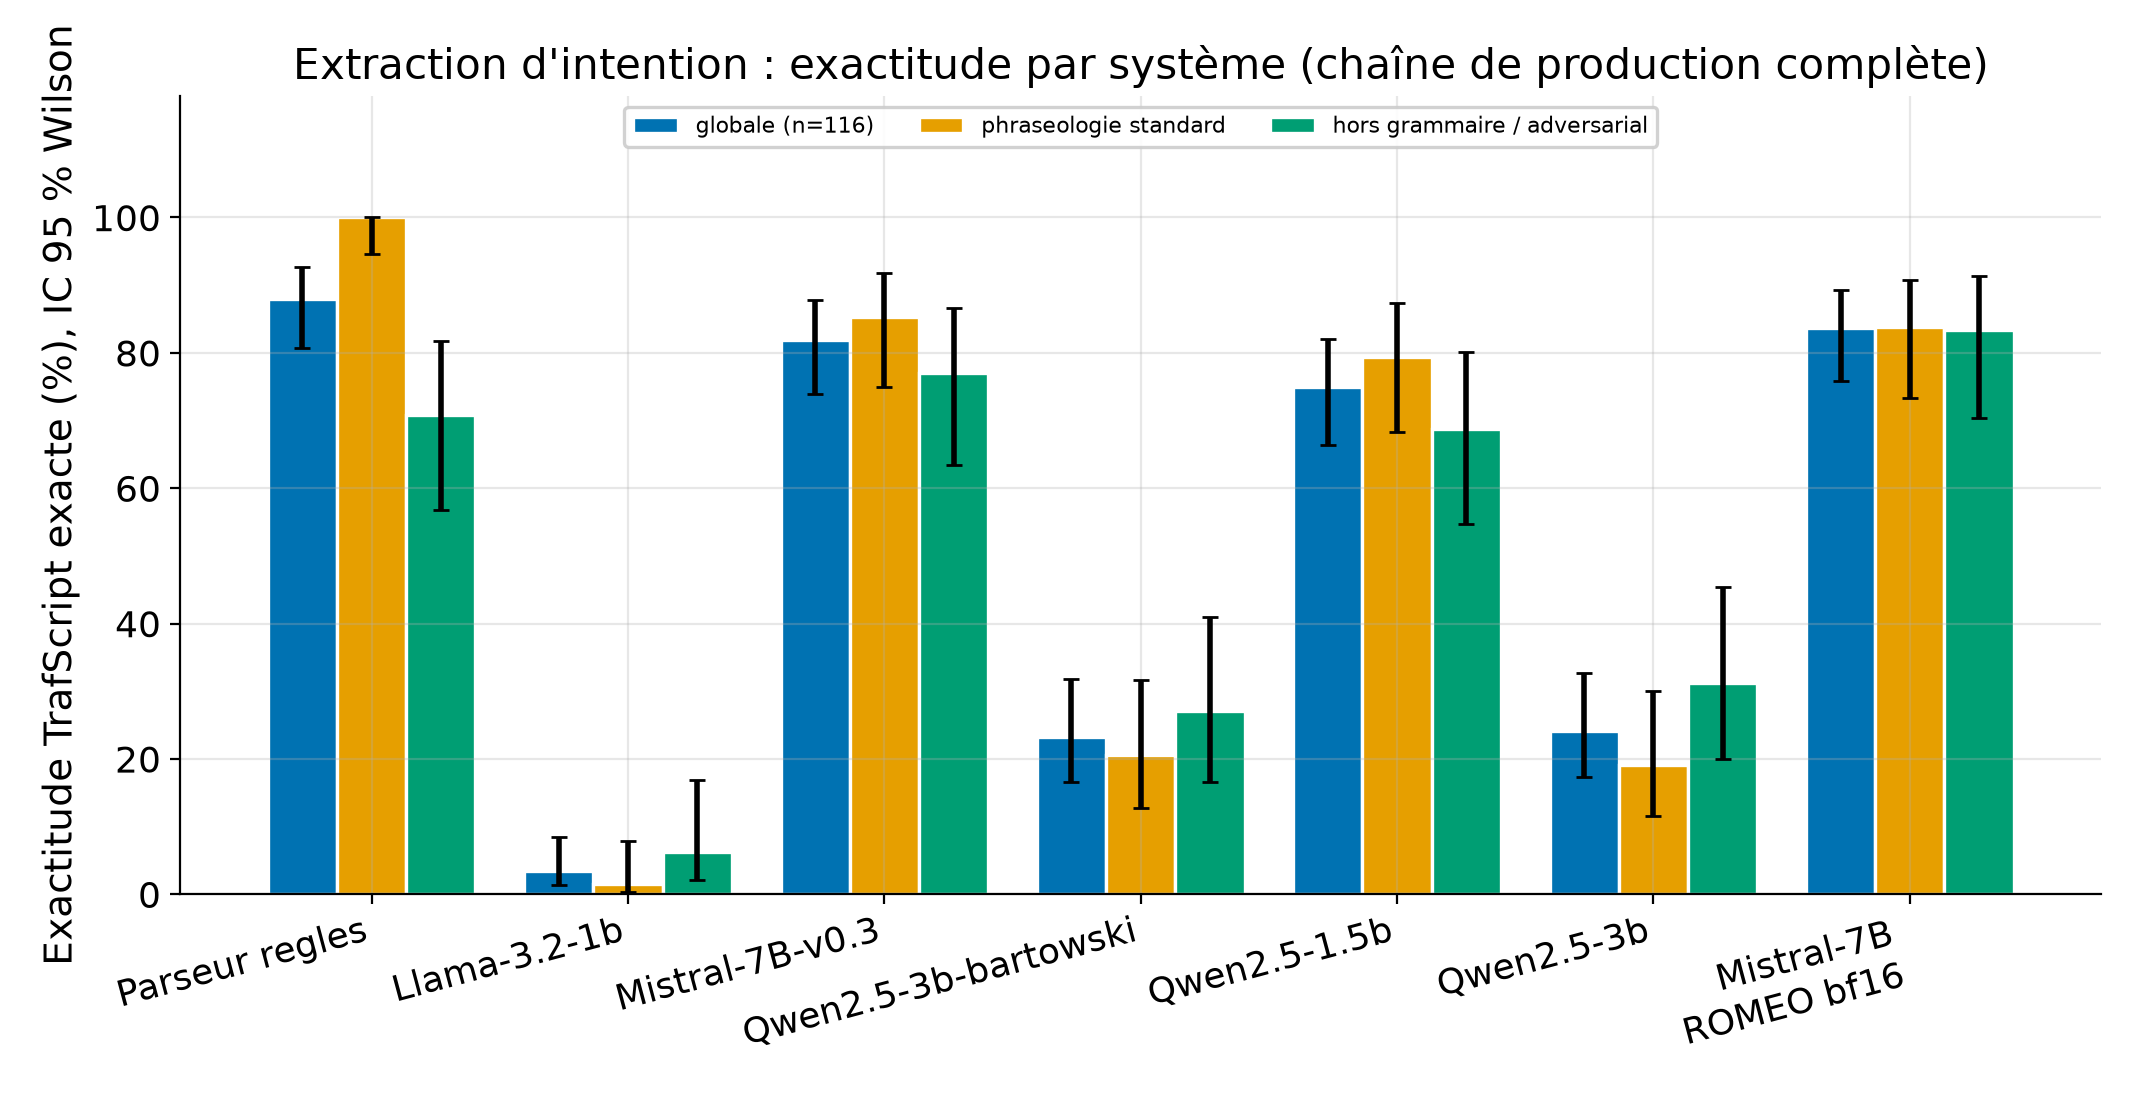
\includegraphics[width=0.96\linewidth, height=0.63\textheight, keepaspectratio]{figures/fig_llm_exactitude.png}

\vspace{3pt}
{\small\textbf{Grammaire fermée} : les règles, 100 \%.
 \enskip$\cdot$\enskip
 \textbf{Hors grammaire} : règles 70,8 \%, modèle \alert{77,1 \%}.\par}
\vspace{1pt}
{\footnotesize\color{ardoise!85} L'écart que le modèle était chargé de
 combler : je garde les deux briques.\par}
\end{frame}

\note{Il n'y a pas de vainqueur mais une complementarite : chaque brique
couvre le regime de langage ou l'autre echoue.
La derniere colonne, Mistral-7B ROMEO, est le meme modele servi en pleine
precision sur le cluster : ne pas la commenter ici, mais si on la remarque,
c'est la diapositive de reserve << ce que coute la quantification 4 bits >>
(83,6 contre 81,9, soit 1,7 point).}

% --- 14. Le prix du langage naturel -----------------------------------------
\begin{frame}{Le prix du langage naturel}
\centering
\vspace{10pt}
\metricsm[ardoise]{45 $\mu$s}{module à base de règles\\\emph{instantané}}
\hspace{12pt}
\metric[bleu]{0,82 s}{Mistral-7B quantifié}
\hspace{12pt}
\metricsm[ardoise]{4,4 Go}{mémoire occupée\\\emph{contre rien}}

\vspace{14pt}
{\small À exactitude équivalente, l'interprétation passe d'un coût
\alert{négligeable} à près d'une seconde. Dans la boucle complète, cet étage
pèse \alert{1,06 s sur 2,6 s}, soit 41 \% du budget : le deuxième poste après
la synthèse vocale.\\
On ne paie ce prix que là où le modèle apporte quelque chose :
\alert{les formulations imprévues}.}

\src{Latences d'interprétation mesurées sur les mêmes 116 clairances
     (\texttt{llm\_bench.json}) ; part dans la boucle mesurée séparément
     (\texttt{e2e\_bench.json}). Les deux systèmes ne sont pas de même nature :
     fonction locale en mémoire contre appel à un serveur d'inférence.}
\end{frame}

\note{Ne PAS annoncer de rapport chiffre entre les deux latences : 0,82 s
contre 45 microsecondes fait un facteur 18 000, c'est arithmetiquement exact
mais ca sonne comme une coquille et ca compare deux natures de systemes, une
fonction locale contre un appel a un serveur. Dire simplement : instantane
d'un cote, presque une seconde de l'autre. Le chiffre qui compte pour le jury
est la part dans la boucle : 41 %. Si on me demande le rapport exact, je peux
le donner (environ 18 000) en precisant qu'il ne mesure pas que le modele.}

% =============================================================================
\section{Les épreuves}

% --- 15. L'enquete : le gabarit ---------------------------------------------
\begin{frame}{L'enquête : le gabarit qui effaçait la consigne}
\centering
\begin{tikzpicture}[scale=0.76, transform shape]

  % ---- rail haut : ce que j'ecris
  \node[etiq, font=\scriptsize\bfseries, text=ardoise, anchor=west] at (-7.6,2.5)
       {CE QUE J'ÉCRIS};
  \node[bloc, minimum width=3.0cm, minimum height=0.9cm, fill=ambre!10,
        draw=ambre!70, text=ambre!75!black] (sys) at (-5.6,1.5)
       {\textsc{système}\\fiches OACI + schéma + sécurité};
  \node[bloc, minimum width=2.3cm, minimum height=0.9cm] (usr) at (-2.2,1.5)
       {\textsc{utilisateur}\\la clairance};
  \node[bloc, minimum width=1.8cm, minimum height=0.9cm, fill=clair] (mo1) at (0.7,1.5)
       {Mistral-7B};
  \draw[fl] (sys.east) -- (usr.west);
  \draw[fl] (usr.east) -- (mo1.west);
  % barre de score 81,9
  \draw[ardoise!40, line width=0.6pt] (2.1,1.15) rectangle (6.6,1.85);
  \fill[vert!55] (2.1,1.15) rectangle (5.79,1.85);
  \node[font=\scriptsize\bfseries, text=vert!55!black, anchor=west] at (6.75,1.5)
       {81,9 \%};
  \draw[fl] (mo1.east) -- (2.05,1.5);

  \draw[ardoise!25, line width=0.5pt] (-7.8,0.55) -- (8.2,0.55);

  % ---- rail bas : ce que le modele recevait
  \node[etiq, font=\scriptsize\bfseries, text=rouge, anchor=west] at (-7.6,-0.1)
       {CE QUE LE MODÈLE RECEVAIT};
  \node[rounded corners=3pt, draw=rouge!60, dashed, line width=0.8pt,
        minimum width=3.0cm, minimum height=0.9cm, align=center,
        font=\tiny, text=rouge!70!black] (sys2) at (-5.6,-1.2)
       {\textsc{système}\\\emph{perdu}};
  \node[bloc, minimum width=2.3cm, minimum height=0.9cm] (usr2) at (-2.2,-1.2)
       {\textsc{utilisateur}\\la clairance};
  \node[bloc, minimum width=1.8cm, minimum height=0.9cm, fill=clair] (mo2) at (0.7,-1.2)
       {Mistral-7B};
  \draw[fl] (usr2.east) -- (mo2.west);
  \draw[flr, dashed] (sys2.south) -- ++(0,-0.75)
        node[etiq, below, text=rouge]{jeté par le gabarit de conversation};
  % barre de score 20,7
  \draw[ardoise!40, line width=0.6pt] (2.1,-1.55) rectangle (6.6,-0.85);
  \fill[rouge!45] (2.1,-1.55) rectangle (3.03,-0.85);
  \node[font=\scriptsize\bfseries, text=rouge!75!black, anchor=west] at (6.75,-1.2)
       {20,7 \%};
  \draw[fl] (mo2.east) -- (2.05,-1.2);
  \node[etiq, text=rouge!80!black, anchor=west] at (2.2,-2.15)
       {et 0 \% de JSON valide};
\end{tikzpicture}

\vspace{4pt}
{\small\textbf{Le modèle n'était pas en cause.} Un test écrit pour ce seul
soupçon : inspecter ce qui part vraiment vers le modèle.}
\src{Correctif : gabarit officiel Mistral, message système fusionné
     $\rightarrow$ 20,7 \% redevient 81,9 \%.}
\end{frame}

\note{Premiers suspects ecartes : la quantification, puis ma propre consigne.
La lecon : un chiffre de benchmark mesure autant l'outil de mesure que le
systeme. Un modele ne s'evalue qu'a travers sa pile de deploiement reelle.}

% --- 16. Trois cas, trois verdicts ------------------------------------------
\begin{frame}{Trois cas, trois verdicts}
\centering
\vspace{6pt}
{\footnotesize
\renewcommand{\arraystretch}{1.5}
\hyphenpenalty=10000\exhyphenpenalty=10000
\begin{tabular}{@{}>{\raggedright\arraybackslash}p{4.4cm} >{\raggedright\arraybackslash}p{3.4cm} >{\raggedright\arraybackslash}p{5.3cm}@{}}
\toprule
\textbf{\color{ardoise}ce que le contrôleur a dit} &
\textbf{\color{ardoise}ce que le modèle propose} &
\textbf{\color{ardoise}verdict de la garde}\\
\midrule
AFR1234, montez niveau 180 &
\texttt{CLIMB FL180} &
\textcolor{vert}{\textbf{ACCEPTÉ}}\\
\emph{transcription bruitée :}\newline « descendez niveau quatre cents »
\newline {\tiny(l'avion est au FL180)} &
\texttt{DESCEND FL400} &
\textcolor{ambre!80!black}{\textbf{REFUSÉ}} \enskip descendre vers un niveau
supérieur\\
direct GOLF ALPHA &
\texttt{ADDWPT GOLFA} &
\textcolor{ambre!80!black}{\textbf{REFUSÉ}} \enskip point absent du secteur\\
\bottomrule
\end{tabular}}

\vspace{10pt}
{\small La garde n'est pas une intention d'architecture : elle est visible et
testable. \emph{L'ordre n'est pas exécuté, le refus est tracé, et l'avion
reste muet : à l'élève de reformuler.}}
\end{frame}

\note{Le jury vient de voir la garde fonctionner sur trois cas concrets, dont
un cas issu d'une vraie transcription deviee.}

% --- 17. Ma garde etait contournable ----------------------------------------
\begin{frame}{Ma garde était contournable}
\centering
\begin{tikzpicture}[scale=0.70, transform shape]
  % mur perce
  \fill[ambre!14, rounded corners=4pt] (-2.1,-2.2) rectangle (2.1,2.2);
  \draw[ambre, line width=1.2pt, rounded corners=4pt] (-2.1,-2.2) rectangle (2.1,2.2);
  \fill[white] (-2.15,-0.9) rectangle (2.15,0.1);   % la breche
  \draw[rouge, dashed, line width=0.9pt] (-2.15,0.1) -- (2.15,0.1);
  \draw[rouge, dashed, line width=0.9pt] (-2.15,-0.9) -- (2.15,-0.9);
  \node[font=\scriptsize\bfseries, text=ambre!75!black] at (0,2.6)
       {VALIDATION DÉTERMINISTE};

  \foreach \y/\t in {1.55/{limites physiques}, 0.75/{cap 0--360},
                     -1.55/{point du secteur}}{
    \node[rounded corners=2pt, fill=white, draw=ambre!55, line width=0.6pt,
          minimum width=3.4cm, minimum height=0.5cm, align=center,
          font=\tiny, text=ardoise] at (0,\y) {\t};}
  \node[bloc, minimum width=2.2cm, minimum height=0.9cm] (llm) at (-5.2,-0.4)
       {ordre du modèle};
  \node[bloc, fill=vert!6, draw=vert!60, minimum width=2.0cm,
        minimum height=0.9cm] (bs) at (5.0,-0.4) {BlueSky};
  \draw[flr, line width=1.6pt] (llm.east) -- (bs.west);
  \node[font=\scriptsize, text=rouge!80!black, align=center] at (0,0.38)
       {cohérence montée / descente};
  \node[font=\scriptsize, text=rouge, fill=white, inner sep=2pt] at (0,-0.42)
       {\emph{brèche} : annoncé bloqué, exécuté quand même};

  % la cause
  \node[rounded corners=3pt, draw=ardoise!45, fill=clair, inner sep=5pt,
        font=\scriptsize\ttfamily, text=ardoise] (cause) at (0,-3.05)
       {"32000.0" \ \textcolor{rouge}{$\neq$} \ "32000"};
  \node[etiq, right=4pt of cause, anchor=west, text=ardoise!80]
       {comparaison de chaînes entre\\la valeur du modèle et la ligne exécutée};
\end{tikzpicture}

\vspace{2pt}
{\small Garde ajoutée en semaine 8 \enskip$\rightarrow$\enskip revue
adversariale un mois plus tard \enskip$\rightarrow$\enskip brèche fermée
et test de non-régression.}
\src{Une garde n'existe vraiment que si quelqu'un a essayé de la casser.}
\end{frame}

\note{L'annonce d'un blocage doit deriver de l'action reellement appliquee,
jamais d'un calcul parallele. C'est le correctif le plus important du stage.}

% --- 18. Le noyau geometrique -----------------------------------------------
\begin{frame}{Le noyau géométrique, lui, se prouve}
\centering
\begin{minipage}[t]{0.52\linewidth}
  \centering
  {\scriptsize\color{ardoise}\textbf{contre une référence numérique}\par}
  \vspace{2pt}
  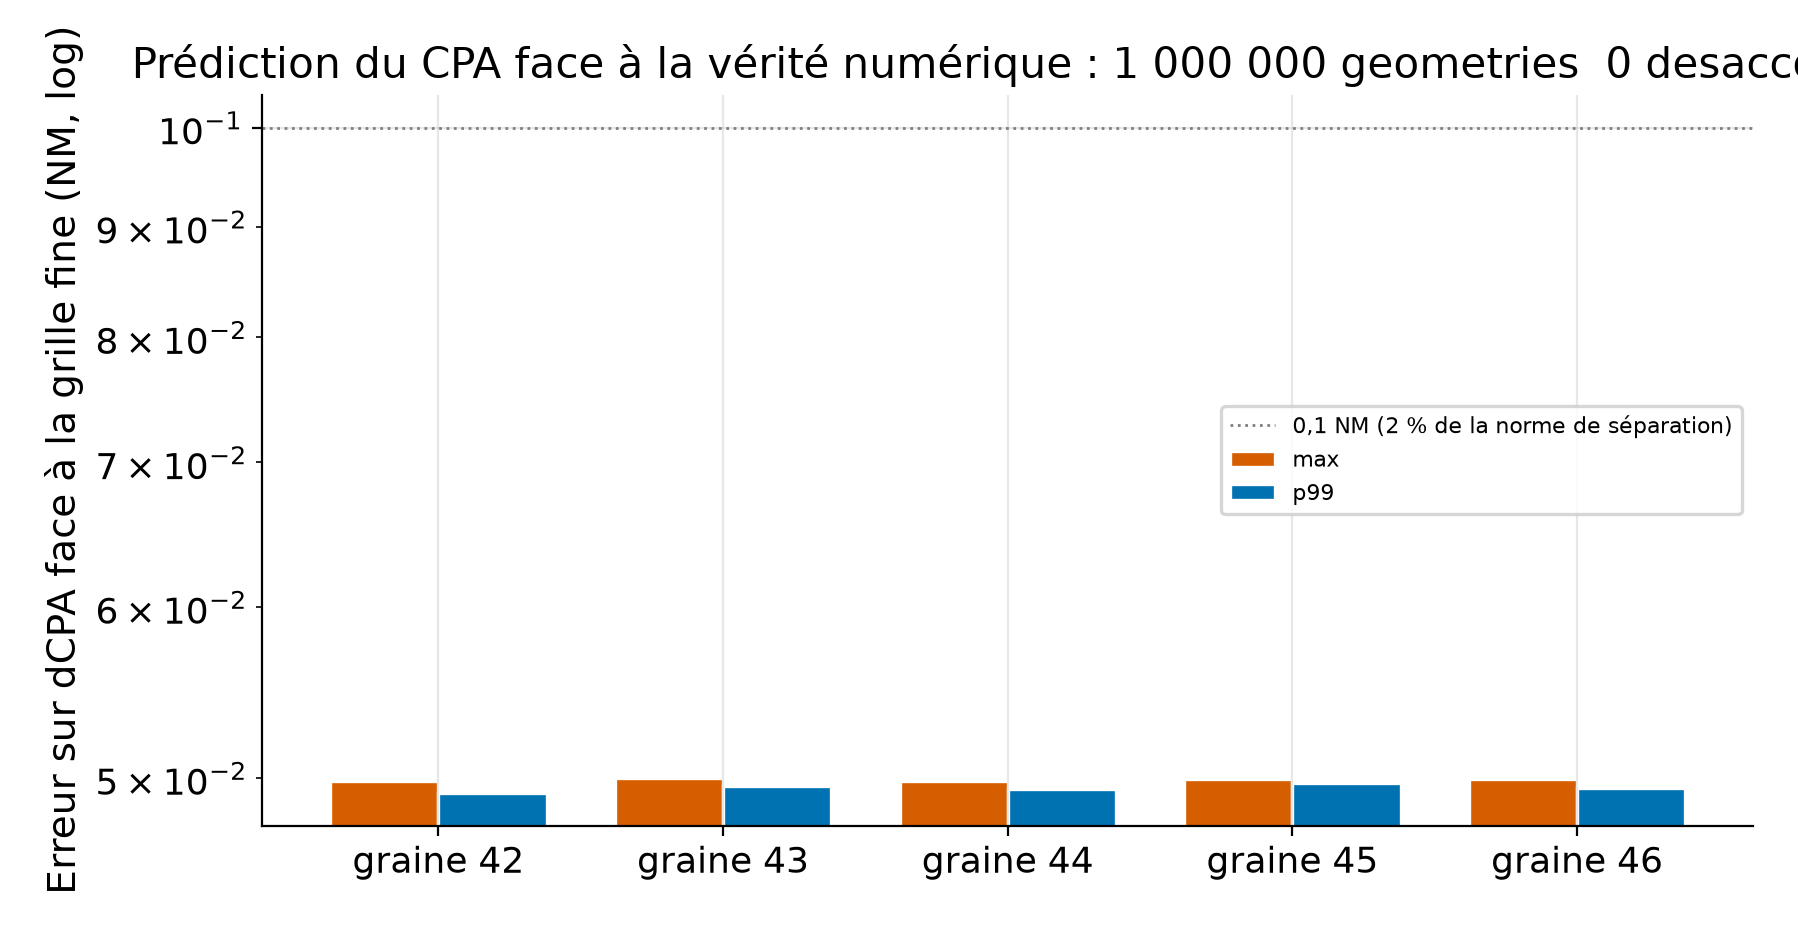
\includegraphics[width=\linewidth, height=0.46\textheight,
                   keepaspectratio]{figures/fig_cpa_multiseed.png}
\end{minipage}
\hfill
\begin{minipage}[t]{0.44\linewidth}
  \centering
  {\scriptsize\color{ardoise}\textbf{contre le simulateur de référence}\par}
  \vspace{2pt}
  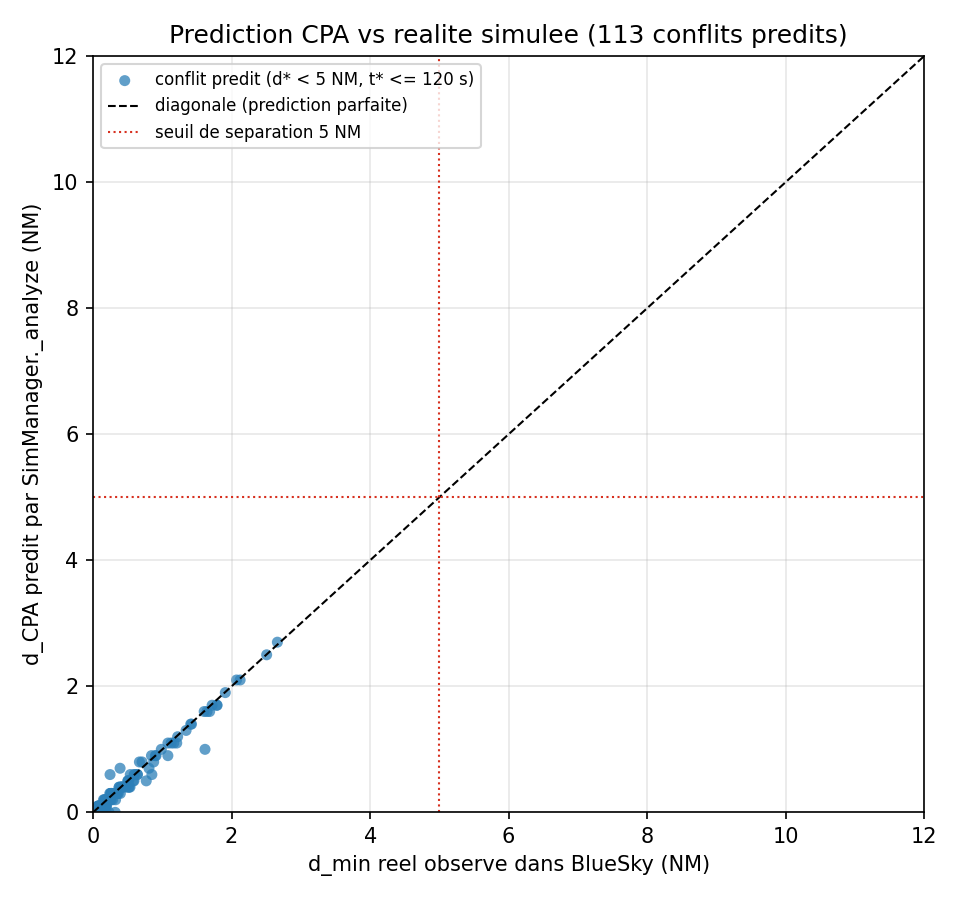
\includegraphics[width=0.78\linewidth, height=0.46\textheight,
                   keepaspectratio]{figures/fig_bluesky_scatter.png}
\end{minipage}

\vspace{4pt}
{\footnotesize
 \textbf{0 désaccord sur 1 000 000} de géométries \enskip$\cdot$\enskip
 erreur maximale \textbf{0,050 NM} \enskip$\cdot$\enskip
 \textbf{aucun conflit manqué, aucune fausse alerte} sur 200 rencontres\par}
\vspace{1pt}
{\scriptsize\color{ardoise!85} C'est ce que résume le score $F_1 = 1{,}00$ : il ne vaut 1 que si le système signale \emph{tous} les conflits réels sans jamais crier au loup.\par}
\vspace{1pt}
{\scriptsize\color{ardoise!85} Accord parfait avec le simulateur de
 référence sur ce protocole, et non une détection parfaite en trafic réel.\par}
\end{frame}

\note{C'est la partie du systeme sur laquelle je peux donner une garantie,
et je la montre : deux verites calculees separement, aucun desaccord.}

% =============================================================================
\section{Répondre, et boucler}

% --- 19. La voix passee a la radio ------------------------------------------
\begin{frame}{On dégrade la voix volontairement}
\centering
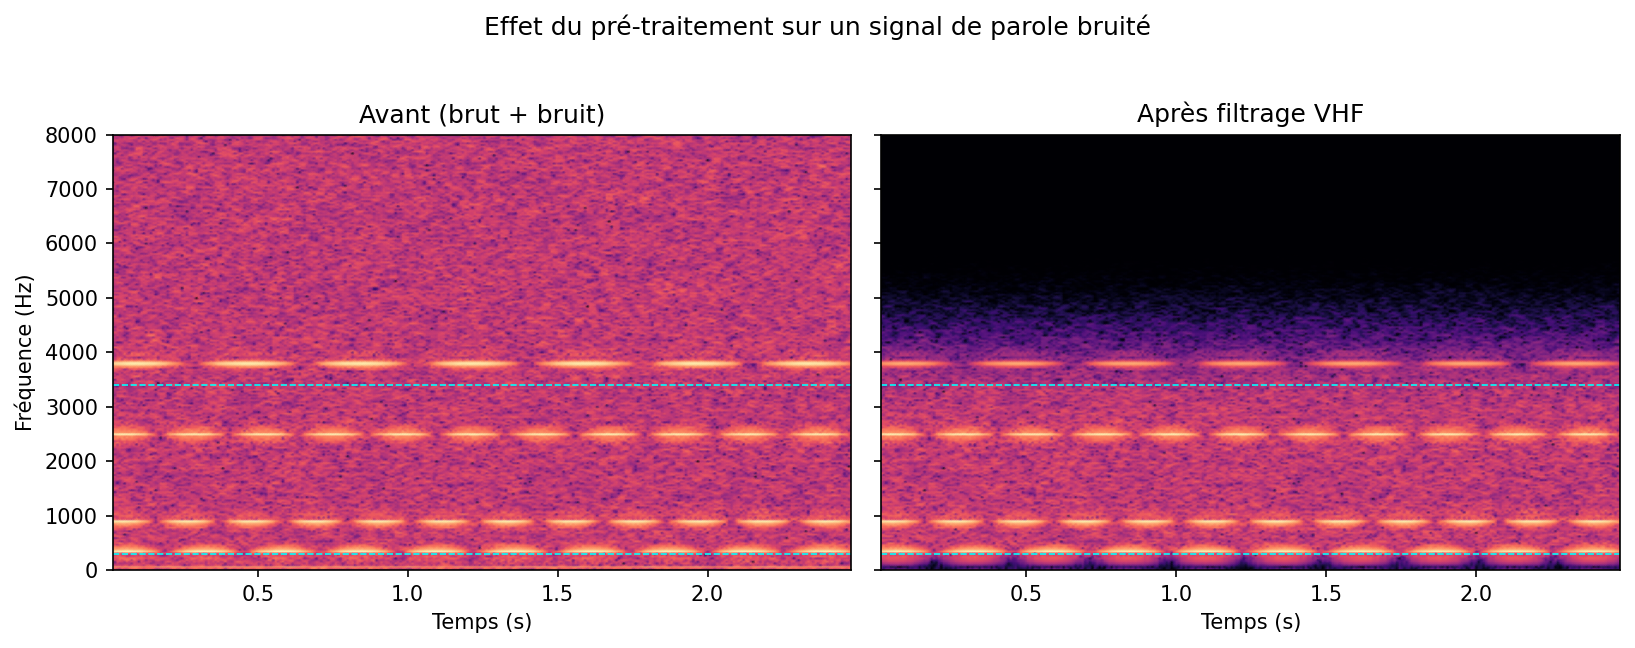
\includegraphics[width=0.64\linewidth, height=0.44\textheight,
                 keepaspectratio]{figures/fig_spectrogramme_avant_apres.png}

\vspace{4pt}
{\footnotesize voix de synthèse \enskip$\longrightarrow$\enskip après le canal
radio VHF : il ne reste que 300--3400 Hz, comme une vraie radio.}

\vspace{5pt}
\metricsm[bleu]{$\times$3 temps réel}{coût de la synthèse}
\hspace{14pt}
\metricsm[ardoise]{le même filtre}{sur l'audio de test \emph{et} sur la voix
  produite}
\end{frame}

\note{Le meme filtre des deux cotes : c'est ce qui rend la mesure honnete.
Et l'eleve doit apprendre a ecouter une mauvaise radio.}

% --- 20. La boucle complete -------------------------------------------------
\begin{frame}{La boucle complète}
\centering
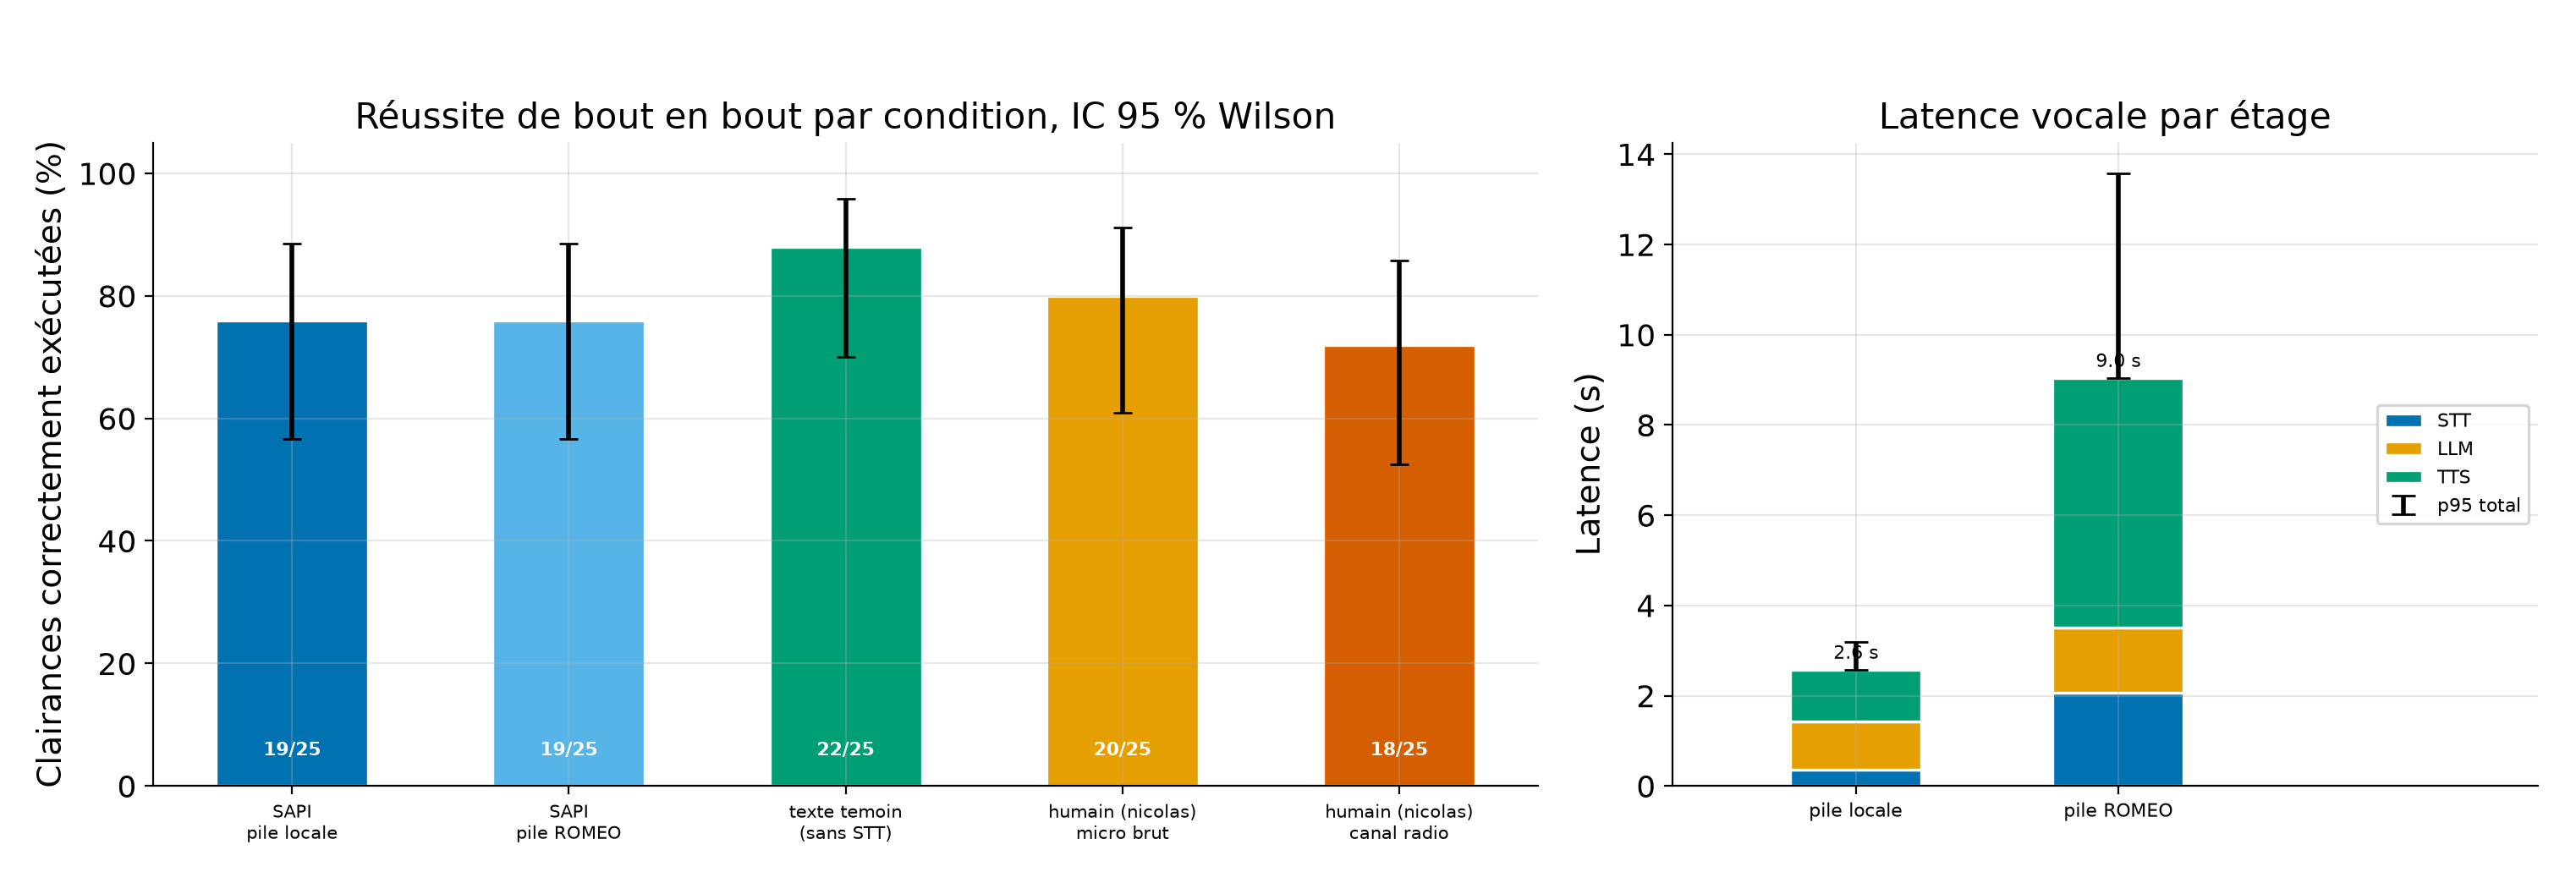
\includegraphics[width=0.98\linewidth, height=0.60\textheight, keepaspectratio, trim=0 0 0 14, clip]{figures/fig_e2e.png}

\vspace{3pt}
{\footnotesize
 \textbf{76 \%} des clairances parlées exécutées correctement (19/25)
 \enskip$\cdot$\enskip témoin clavier 88 \%
 \enskip$\cdot$\enskip ma propre voix : \textbf{80 \%} au micro\par}
\vspace{1pt}
{\scriptsize\color{ardoise!85} 25 cas par condition, intervalles larges et
 recouvrants \enskip$\cdot$\enskip contre-épreuve humaine : un seul
 locuteur.\par}
\end{frame}

\note{La question d'origine recoit une reponse chiffree, y compris face a une
vraie voix. J'annonce moi-meme les limites de l'echantillon avant qu'on me
les oppose.}

% --- 21. ROMEO tombe --------------------------------------------------------
\begin{frame}{Le supercalculateur tombe, la campagne continue}
\centering
\begin{tikzpicture}[scale=0.84, transform shape]
  \node[bloc, minimum width=3.0cm, minimum height=1.3cm] (app) at (-5.6,0)
       {application\\+ banc de mesure};
  \node[rounded corners=3pt, fill=bleu!8, draw=bleu!55, line width=0.9pt,
        minimum width=1.0cm, minimum height=4.2cm, align=center,
        font=\tiny, text=bleu] (api) at (-2.4,0)
       {contrat\\unique\\\textsc{api}\\\textsc{openai}};
  \draw[fl] (app.east) -- (api.west);

  \node[bloc, minimum width=3.2cm, minimum height=0.95cm, fill=rouge!5,
        draw=rouge!55, text=rouge!70!black] (romeo) at (2.4,1.55)
       {ROMEO \enskip GH200 \enskip aarch64};
  \node[bloc, minimum width=3.2cm, minimum height=0.95cm, fill=vert!6,
        draw=vert!60, text=vert!55!black] (local) at (2.4,0)
       {GPU portable \enskip RTX 4070};
  \node[bloc, minimum width=3.2cm, minimum height=0.95cm, dashed,
        text=ardoise!70] (cloud) at (2.4,-1.55) {service distant};

  \draw[fl, rouge!60] (api.east) -- (romeo.west);
  \draw[flg] (api.east) -- (local.west);
  \node[font=\tiny, text=vert!55!black, align=center, fill=white,
        inner sep=1.5pt] at (-0.55,-0.42) {une ligne\\de configuration};
  \draw[fl, ardoise!40, dashed] (api.east) -- (cloud.west);

  % l'eclair
  \draw[rouge, line width=1.6pt] (4.55,2.15) -- (4.15,1.55) -- (4.55,1.55) -- (4.15,0.95);
  \node[etiq, text=rouge!80!black, anchor=west] at (4.95,1.55)
       {indisponibilité totale,\\en pleine campagne de mesure};

  \node[etiq, below=6pt of cloud, text=ardoise!70]
       {décision prise trois semaines plus tôt\\pour rendre les pannes visibles};
\end{tikzpicture}

\vspace{4pt}
{\small Un choix d'architecture pris pour une raison a été validé par un
incident qu'il n'anticipait pas.}
\end{frame}

\note{Quota de 20 Go par partition, architecture ARM exotique, bug cuFFT sur
la synthese vocale : le cluster a coute cher en ingenierie. Et quand il est
tombe, une ligne de configuration a suffi.}

% =============================================================================
\section{Bilan}

% --- 22. Perimetre assume ---------------------------------------------------
\begin{frame}{Périmètre assumé}
\centering
\vspace{4pt}
\begin{tikzpicture}[scale=0.88, transform shape,
  carte/.style={rounded corners=3pt, draw=ardoise!40, fill=ardoise!4,
                line width=0.7pt, text width=5.6cm, minimum height=1.25cm,
                align=left, font=\scriptsize, text=ardoise, inner sep=8pt}]
  \node[carte] (c1) at (-3.35,1.0)
       {\textbf{\large $n = 1$}\\un seul locuteur humain, 25 phrases :
        aucune évaluation par des contrôleurs};
  \node[carte] (c2) at (3.35,1.0)
       {\textbf{\large 25 cas}\\intervalles de confiance de l'ordre de
        $\pm 15$ points en bout de chaîne};
  \node[carte] (c3) at (-3.35,-0.95)
       {\textbf{\large 116 clairances}\\un secteur fictif à 7 points,
        une langue, une phraséologie};
  \node[carte] (c4) at (3.35,-0.95)
       {\textbf{\large 1 machine}\\RTX 4070 Laptop 8 Go : les latences ne se
        transposent pas};
\end{tikzpicture}

\vspace{10pt}
\cle{Un banc d'essai, pas une validation opérationnelle.}
\end{frame}

\note{Enoncer moi-meme les limites, chiffrees, desamorce la moitie des
questions et fait partie de la demonstration de rigueur.}

% --- 23. Ce qu'il faut retenir ----------------------------------------------
\begin{frame}{Ce qu'il faut retenir}
\centering
\begin{tikzpicture}[scale=0.86, transform shape]
  \def\dx{2.85}
  \node[blocia, minimum width=2.3cm, minimum height=1.2cm] (b1) at (0,0)
       {\textbf{ENTENDRE}};
  \node[blocia, minimum width=2.3cm, minimum height=1.2cm] (b2) at (\dx,0)
       {\textbf{COMPRENDRE}};
  \node[bloccode, minimum width=2.3cm, minimum height=1.55cm] (b3) at (2*\dx,0)
       {\textbf{VÉRIFIER}};
  \node[bloc, minimum width=2.3cm, minimum height=1.2cm] (b4) at (3*\dx,0)
       {\textbf{EXÉCUTER}};
  \node[blocia, minimum width=2.3cm, minimum height=1.2cm] (b5) at (4*\dx,0)
       {\textbf{RÉPONDRE}};
  \foreach \i/\j in {1/2, 2/3, 3/4, 4/5}{\draw[fl] (b\i) -- (b\j);}

  \node[etiq, below=4pt of b1, text=ardoise]
       {\textbf{\normalsize 28,5 \%}\\d'erreur mots\\\emph{contre 71,9 \%}};
  \node[etiq, below=4pt of b2, text=ardoise]
       {\textbf{\normalsize 81,9 \%}\\indiscernable\\du parseur};
  \node[etiq, below=8pt of b3, text=ambre!80!black]
       {\textbf{\large 0}\\sortie de modèle\\non vérifiée};
  \node[etiq, below=4pt of b4, text=ardoise]
       {\textbf{\normalsize 0 désaccord}\\sur $10^6$\\géométries};
  \node[etiq, below=4pt of b5, text=ardoise]
       {\textbf{\normalsize 76 \%}\\boucle complète\\en 2,6 s};

  \draw[fl, bleu] (b5.east) -- (13.0,0) -- (13.0,-2.95) -- (-2.5,-2.95)
                  -- (-2.5,0) -- (b1.west);
\end{tikzpicture}

\vspace{4pt}
\begin{tikzpicture}
  \node[rounded corners=3pt, fill=ambre!16, draw=ambre, line width=1pt,
        inner sep=8pt, minimum width=12.5cm, align=center] {
    {\large\bfseries\color{ambre!75!black} LE MODÈLE PROPOSE, LE CODE VÉRIFIE}};
\end{tikzpicture}

\vspace{4pt}
{\scriptsize\color{ardoise!80} Suites : plusieurs locuteurs et accents
 \enskip$\cdot$\enskip phraséologie française et secteurs multiples
 \enskip$\cdot$\enskip évaluation par des élèves contrôleurs}
\end{frame}

\note{Le jury repart capable de redessiner la chaine lui-meme et de dire
pourquoi la boite ambre, et non un score de modele, est le vrai resultat du
stage.}

% --- Merci ------------------------------------------------------------------
\bgimage{figures/demo_radar_live.png}{0.74}
\begin{frame}[plain]
  \vfill
  \centering
  {\color{white}\fontsize{30}{34}\selectfont\bfseries Merci de votre attention\par}
  \vspace{6pt}
  \textcolor{ambre}{\rule{40mm}{1.4pt}}\\[12pt]
  {\color{white!80}\small
   Code, corpus annotés, protocoles et résultats bruts :\\[2pt]
   \texttt{github.com/Gotman08/simulateur-controleur-aerien}\par}
  \vfill
\end{frame}
\bgclear

% =============================================================================
\appendix

\bgfill{bleu}
\begin{frame}[plain]
  \vfill
  \centering
  {\color{white}\fontsize{26}{30}\selectfont\bfseries Diapositives de réserve\par}
  \vspace{6pt}
  \textcolor{ambre}{\rule{38mm}{1.4pt}}
  \vfill
\end{frame}
\bgclear

\begin{frame}{Réserve : exactitude par catégorie de clairance}
\centering
\vfill
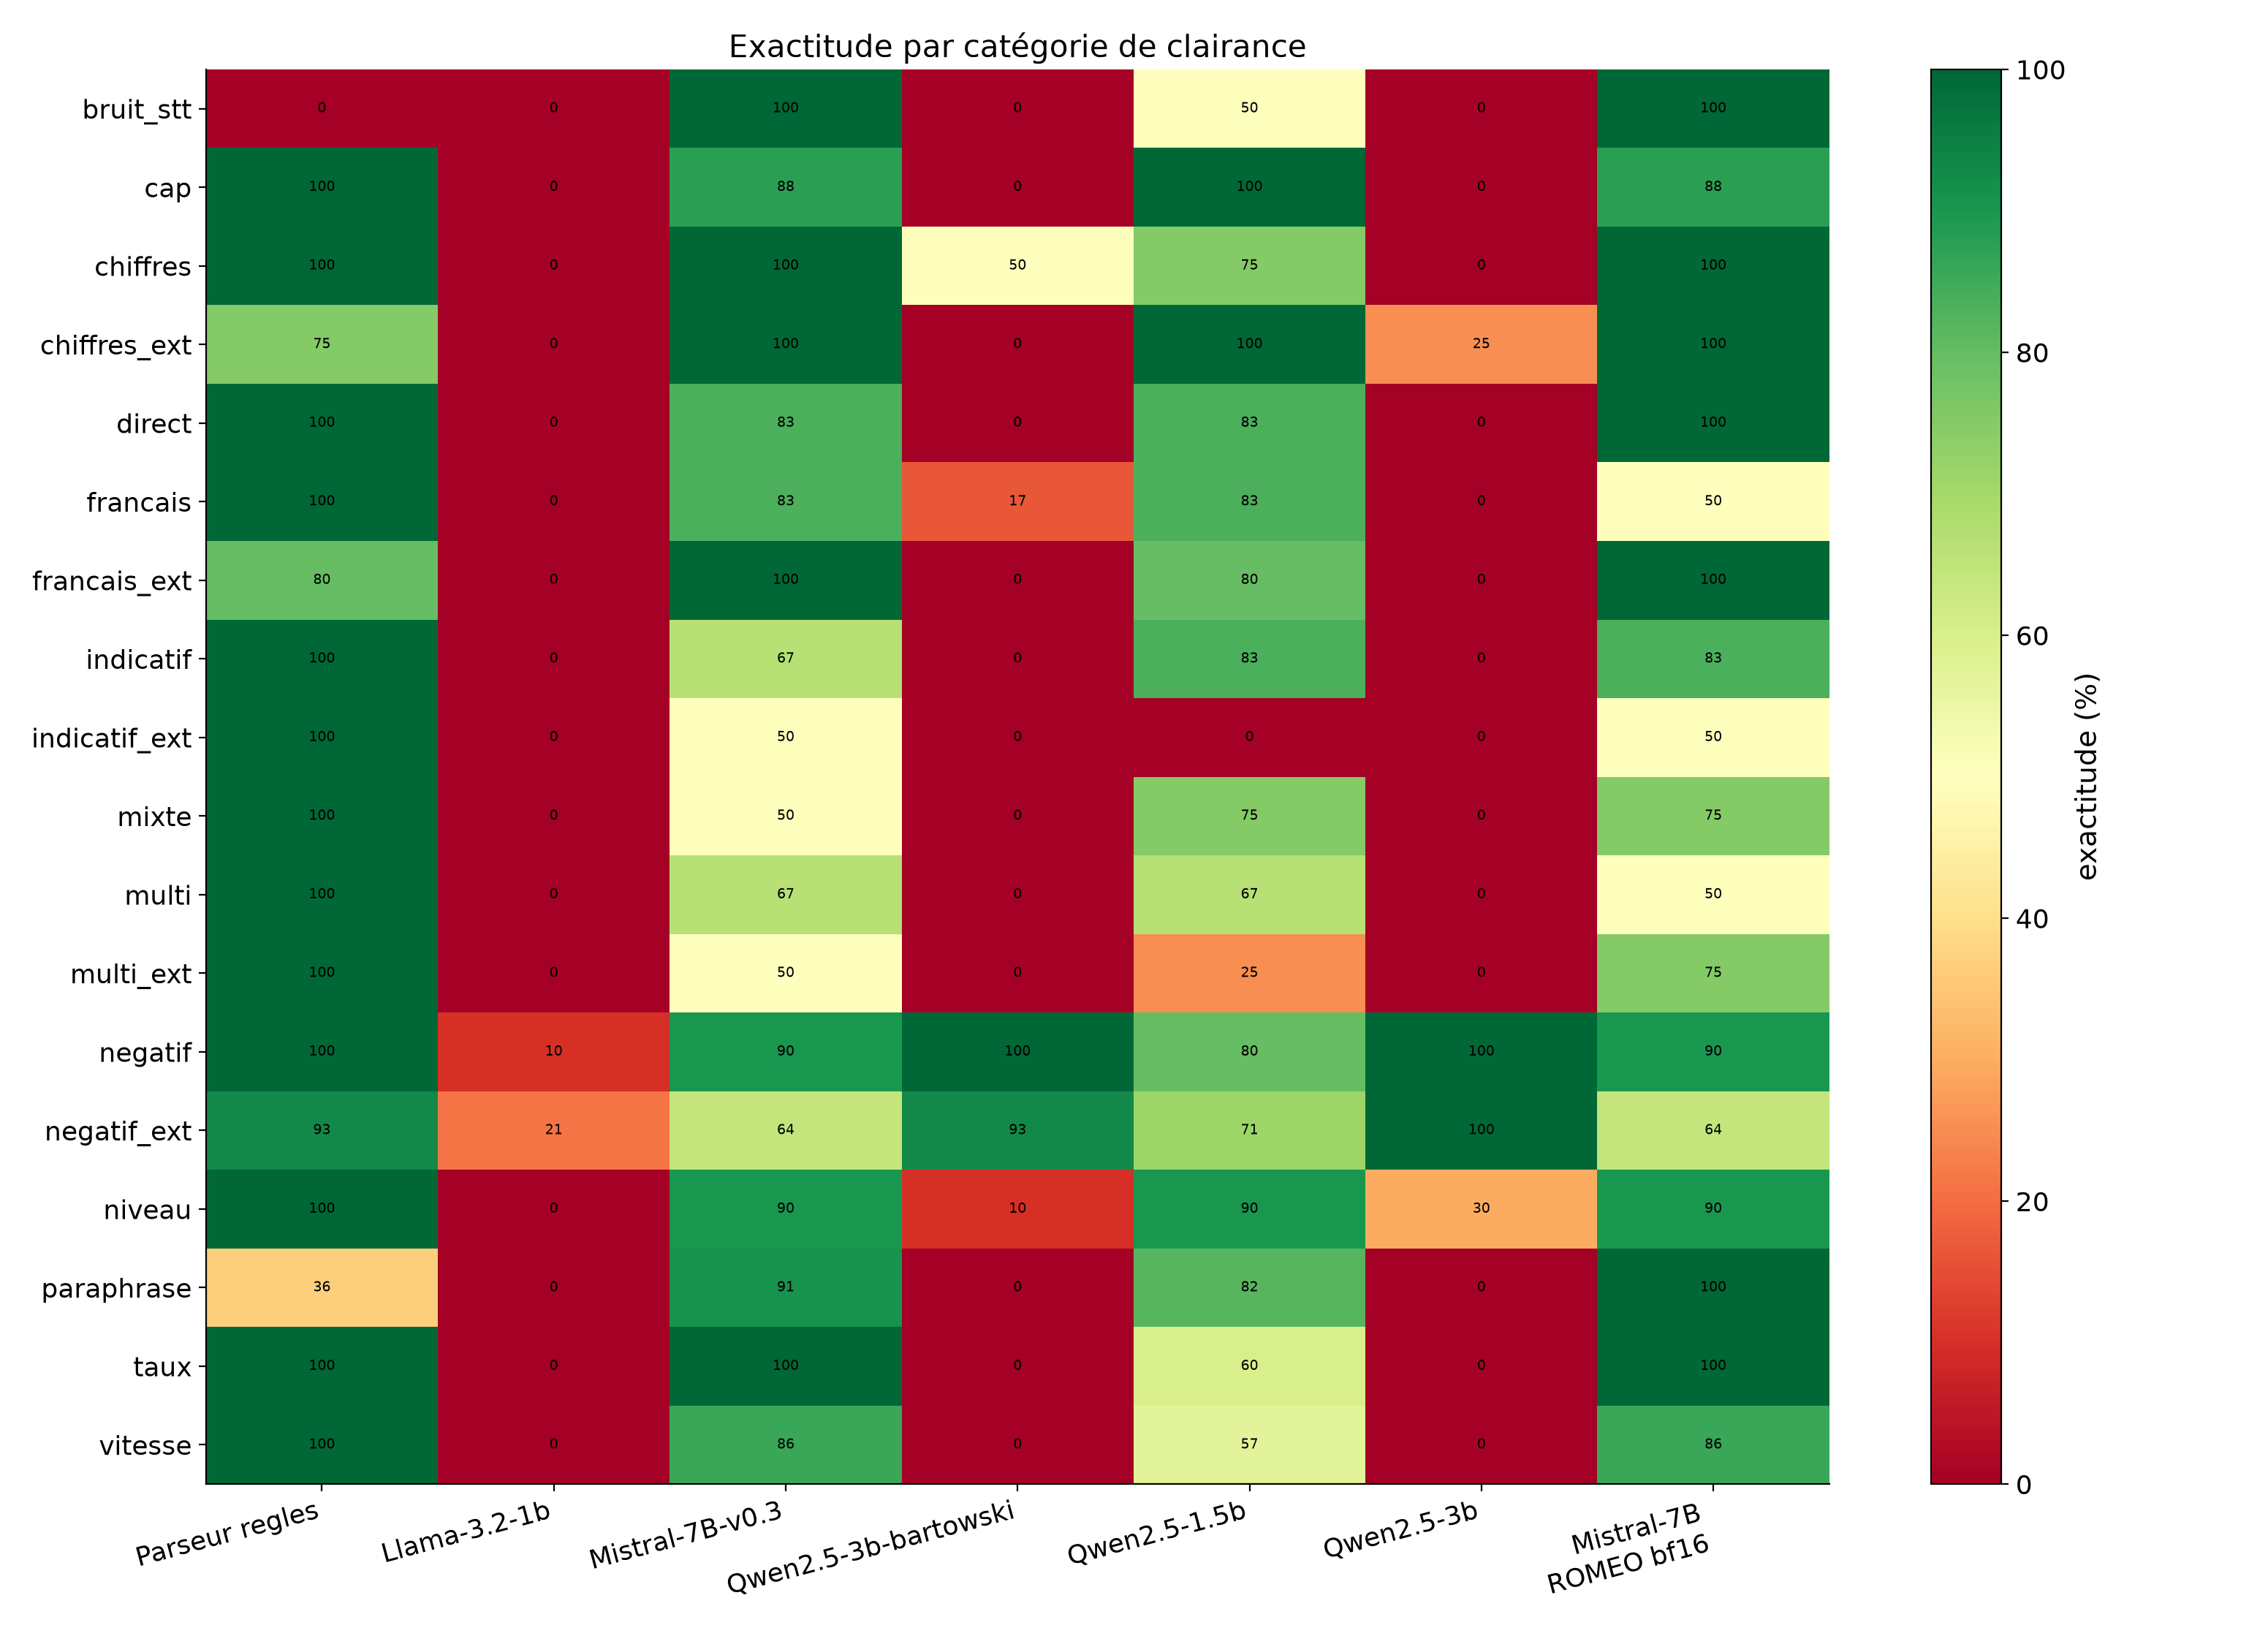
\includegraphics[width=\linewidth, height=0.82\textheight, keepaspectratio]{figures/fig_llm_categories.png}
\vfill
\end{frame}

\begin{frame}{Réserve : latence et débit des modèles locaux}
\centering
\vfill
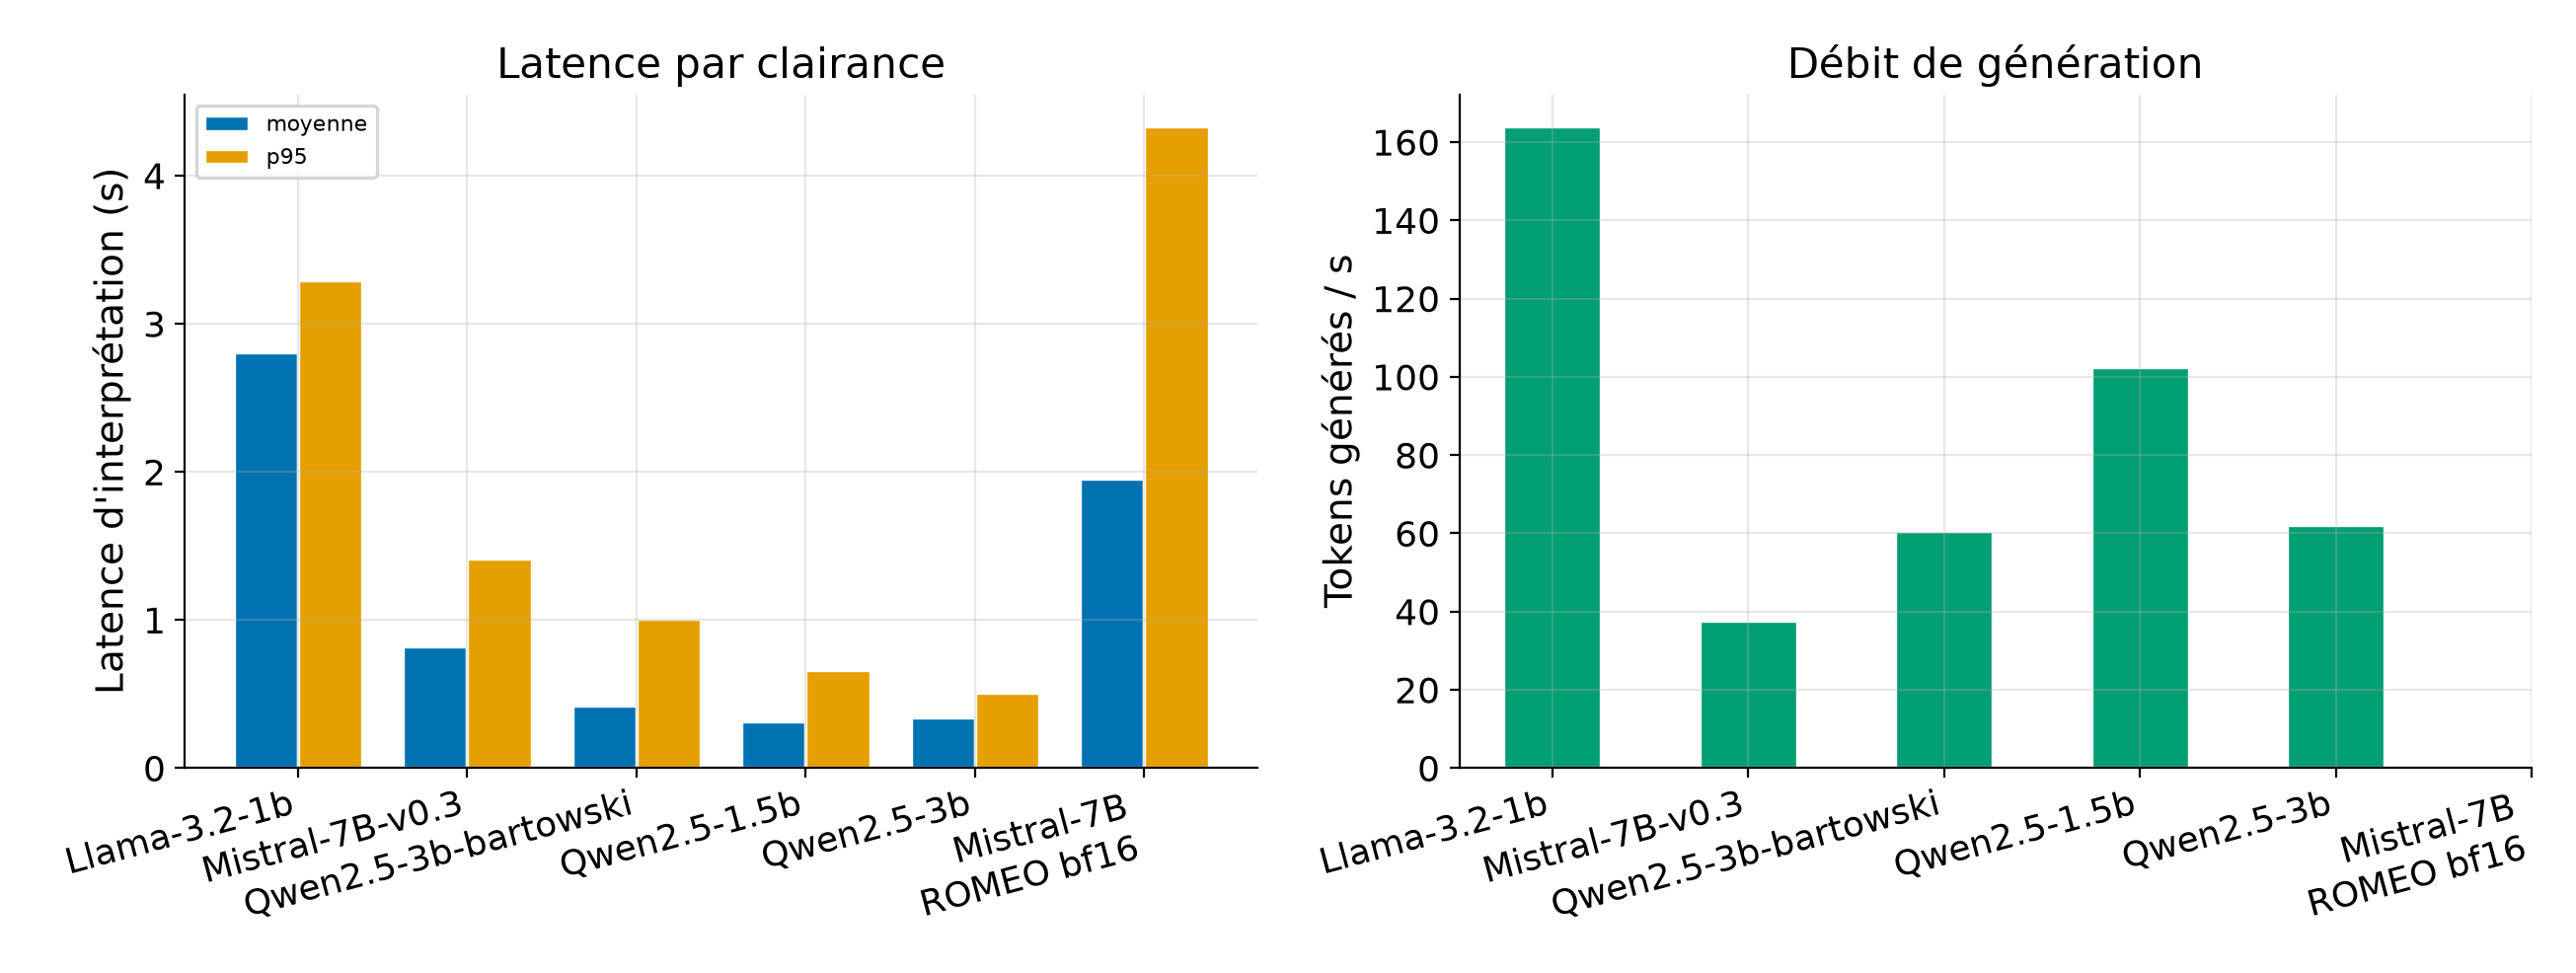
\includegraphics[width=0.98\linewidth, height=0.76\textheight, keepaspectratio]{figures/fig_llm_latence.png}
\vfill
\end{frame}

\begin{frame}{Réserve : coût et intelligibilité de la synthèse vocale}
\centering
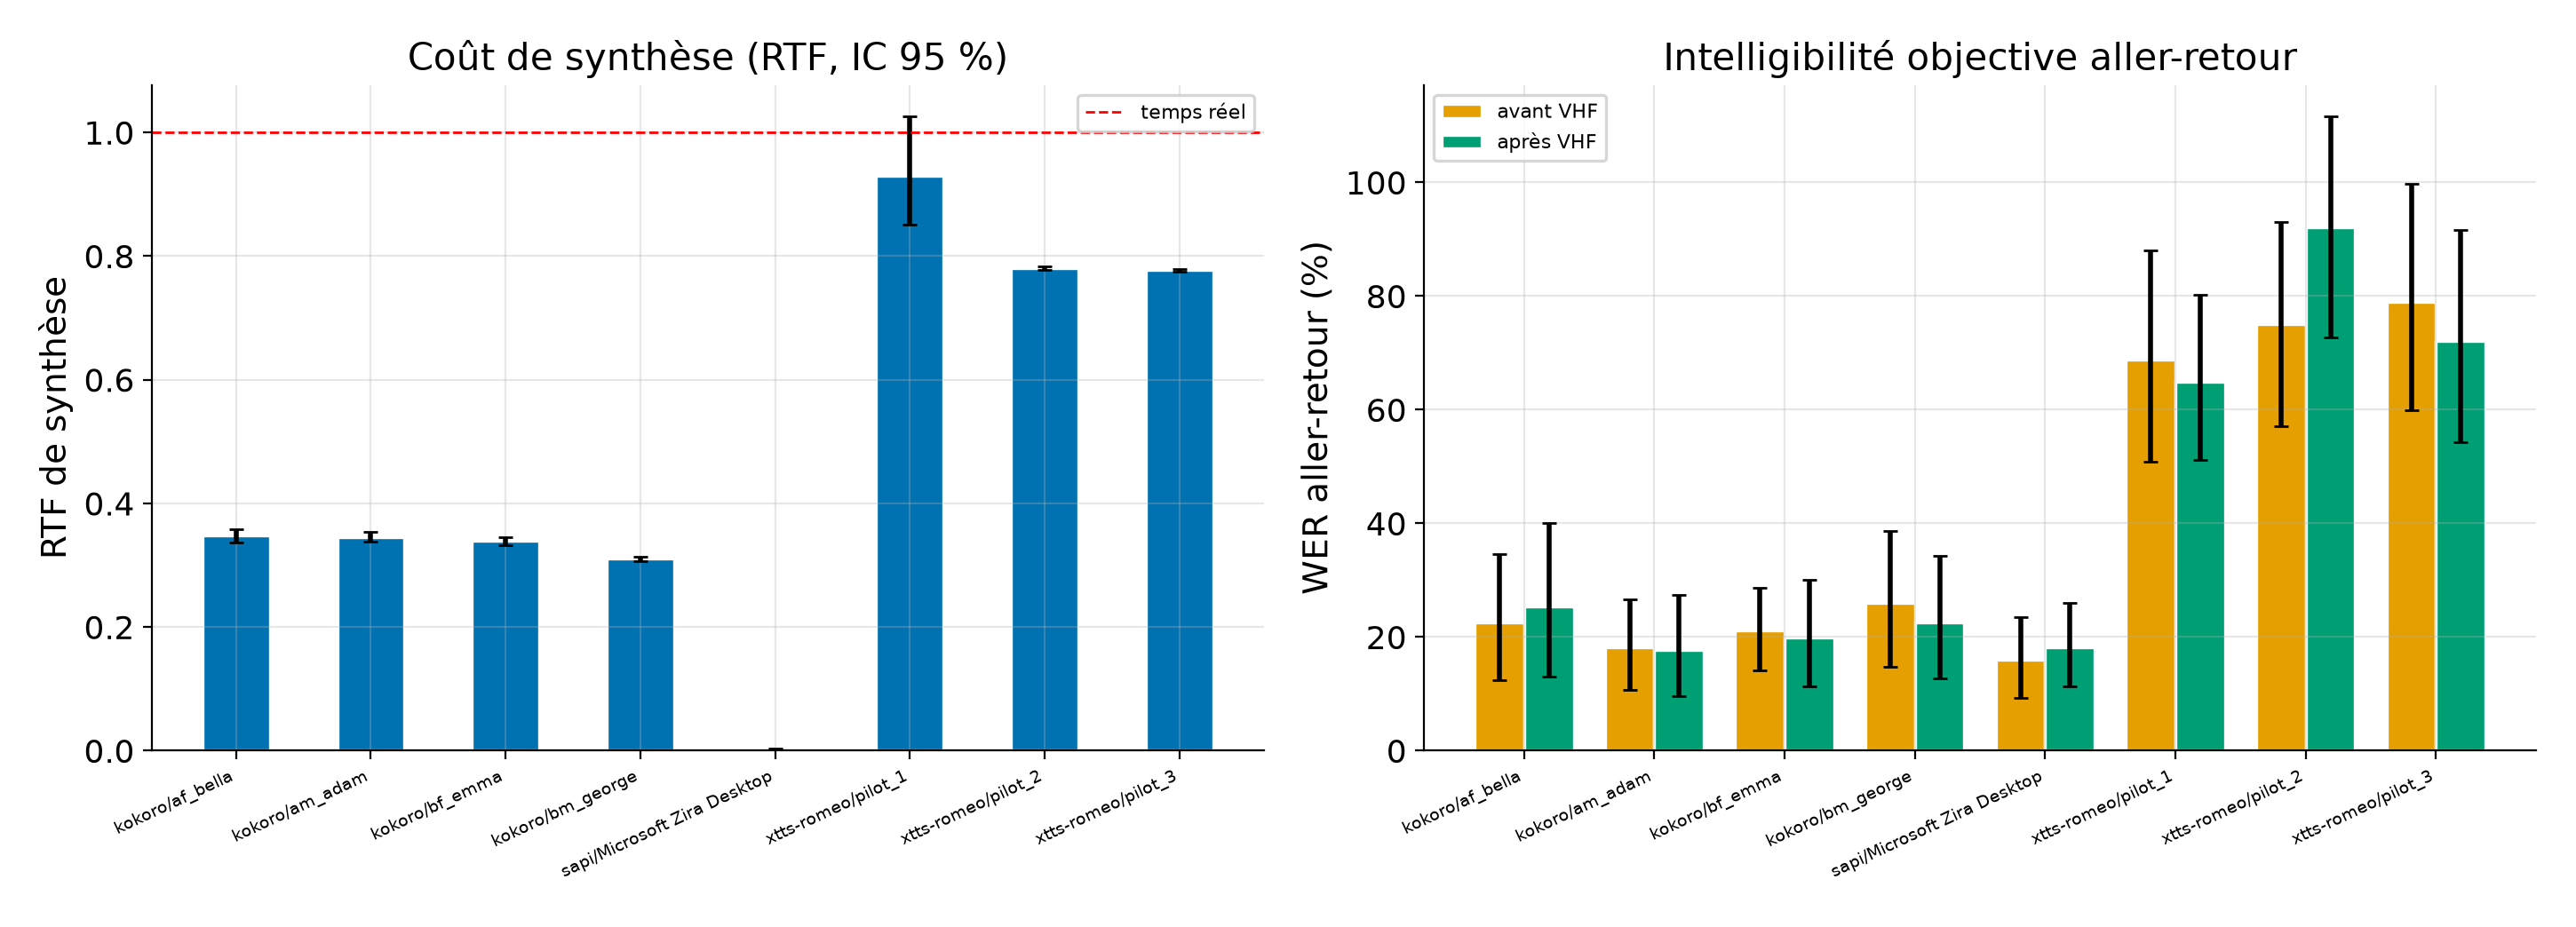
\includegraphics[width=1.0\linewidth, height=0.64\textheight, keepaspectratio]{figures/fig_tts.png}

\vspace{2pt}
{\footnotesize Les trois barres de droite sont les voix \textbf{clonées} XTTS
 servies depuis le cluster : \alert{65 à 92 \% de WER aller-retour} contre 18 à
 25 \% pour Kokoro. Le clonage part d'extraits radio déjà dégradés et reproduit
 fidèlement la dégradation.}
\end{frame}

\begin{frame}{Réserve : ce que coûte la quantification 4 bits}
\centering
\vspace{6pt}
\metric[ardoise]{83,6 \%}{Mistral-7B \textbf{non compressé}\\sur ROMEO, 14,5 Go}
\hspace{16pt}
\metric[bleu]{81,9 \%}{Mistral-7B \textbf{Q4\_K\_M}\\en local, 4,4 Go}

\vspace{12pt}
\begin{block}{1,7 point d'exactitude}
  \centering
  Le même modèle, les mêmes 116 clairances : compresser par quatre coûte
  \alert{1,7 point}, et divise la latence par 2,4.
\end{block}

\src{\texttt{bench/results/llm\_bench.json} et \texttt{llm\_bench\_romeo.json}}
\end{frame}

\begin{frame}{Réserve : pourquoi pas le petit modèle ?}
\centering
\vspace{6pt}
\metric[bleu]{81,9 \%}{Mistral-7B \enskip$\cdot$\enskip 0,82 s}
\hspace{16pt}
\metric[ardoise]{75,0 \%}{Qwen2.5-1.5B \enskip$\cdot$\enskip 0,32 s}

\vspace{12pt}
\begin{block}{McNemar apparié : $p = 0{,}15$}
  \centering
  L'écart de 6,9 points \alert{n'est pas significatif} sur 116 cas.
\end{block}

\vspace{6pt}
{\footnotesize Je garde Mistral pour deux raisons qui ne sont pas l'exactitude
 globale : 100 \% de JSON strictement valide contre 96,6 \%, et il est le seul des
 deux à battre le module à règles \emph{hors} grammaire (77,1 contre 68,8 \%).}

\src{Sur un corpus plus grand, la question mériterait d'être rouverte.}
\end{frame}

\begin{frame}{Réserve : pourquoi pas un modèle vocal de bout en bout ?}
\centering
\vspace{4pt}
\metric[ardoise]{36 \%}{collationnements corrects\\VoiceChat-11B, voix de synthèse}
\hspace{16pt}
\metric[rouge]{0 \%}{ordres exacts\\dans les \textbf{quatre} conditions}

\vspace{12pt}
\begin{block}{Le modèle converse, il n'exécute pas}
  \centering
  Battu par la cascade dans les quatre conditions
  ($p_{\text{Holm}}$ de 0,001 à 0,008).
\end{block}

\vspace{4pt}
{\footnotesize Dans une cascade, on peut insérer une couche de vérification
 entre la compréhension et l'action. Dans un modèle de bout en bout,
 \alert{il n'y a pas d'endroit où la mettre}.}

\src{NVIDIA VoiceChat-11B sur GH200, 25 clairances $\times$ 4 conditions
     \enskip$\cdot$\enskip \texttt{bench/results/voicechat\_romeo.json}}
\end{frame}

\begin{frame}{Réserve : montée en charge du simulateur}
\centering
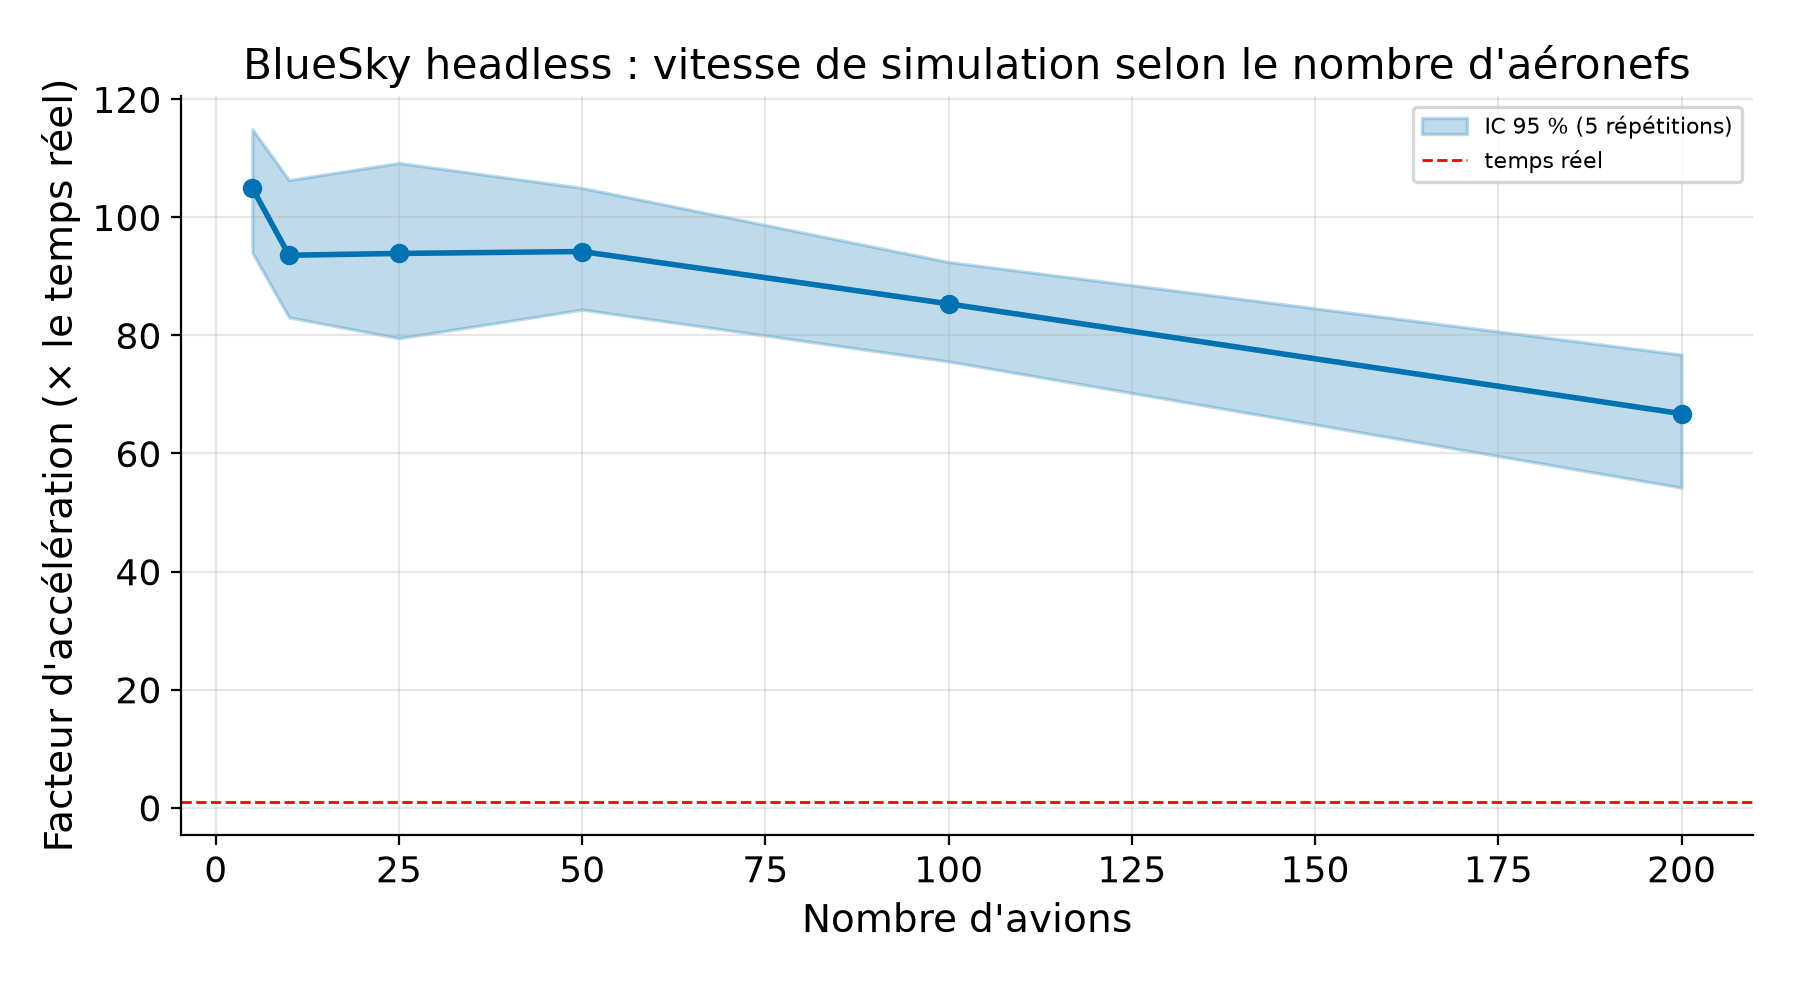
\includegraphics[width=0.74\linewidth, height=0.56\textheight, keepaspectratio]{figures/fig_sim_scaling.png}

\vspace{2pt}
{\footnotesize L'axe vertical est un \textbf{facteur d'accélération} : à 200
 aéronefs, le simulateur avance le trafic 67 fois plus vite que l'horloge,
 autrement dit simuler \textbf{1 seconde} de trafic lui coûte \textbf{15 ms}
 de calcul.}
\end{frame}

\begin{frame}{Réserve : conflits garantis par construction}
\centering
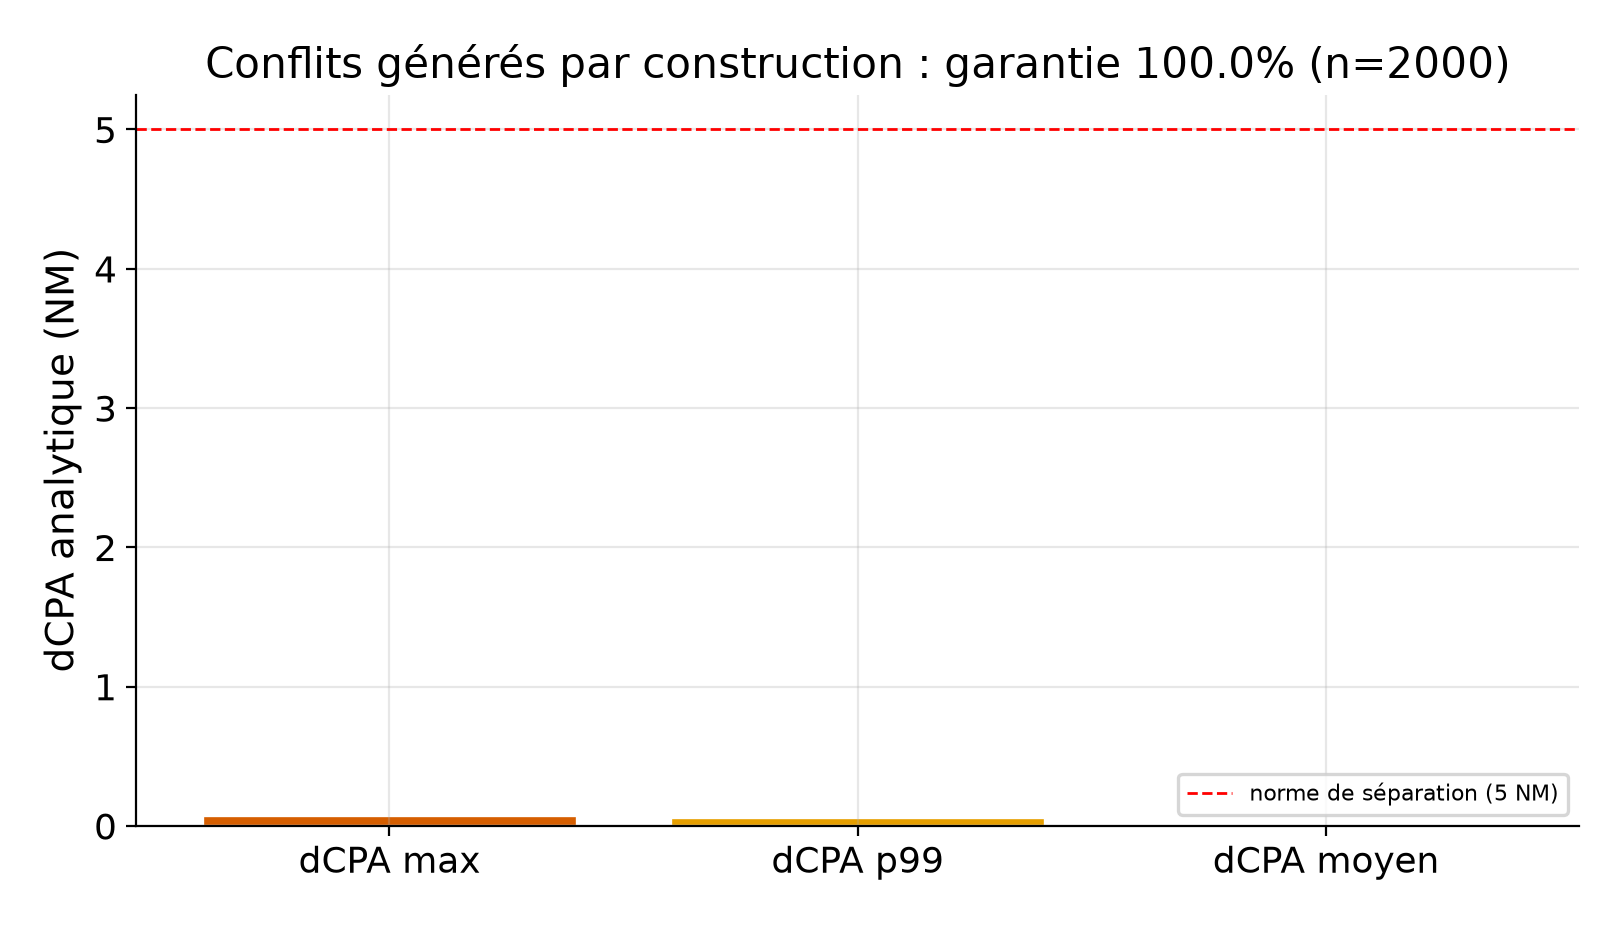
\includegraphics[width=0.66\linewidth, height=0.58\textheight, keepaspectratio]{figures/fig_conflit_garanti.png}

\vspace{2pt}
{\footnotesize 2 000 tirages seedés, garantie vérifiée à 100 \%
 ($d_{CPA}$ maximal 0,082 NM $\ll$ 5 NM).}
\end{frame}

\begin{frame}{Réserve : le filtre VHF}
\centering
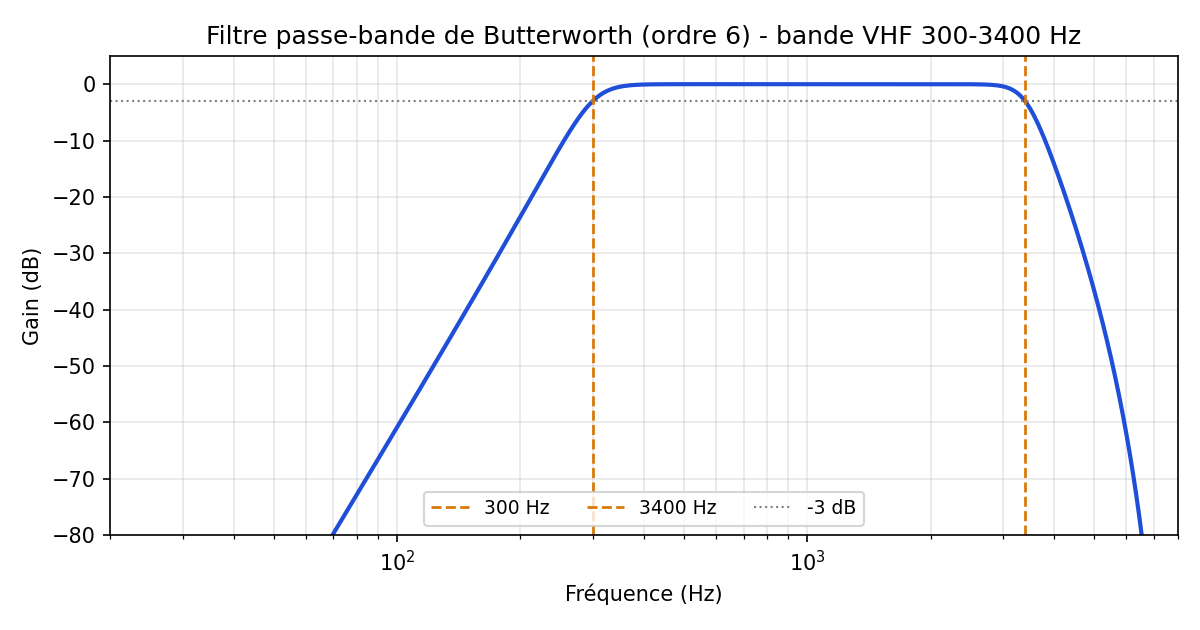
\includegraphics[width=0.74\linewidth, height=0.58\textheight, keepaspectratio]{figures/fig_butterworth_bode.png}

\vspace{2pt}
{\footnotesize Passe-bande de Butterworth d'ordre 6, 300--3400 Hz.}
\end{frame}

\begin{frame}{Réserve : le mode exercice et son débriefing}
\centering
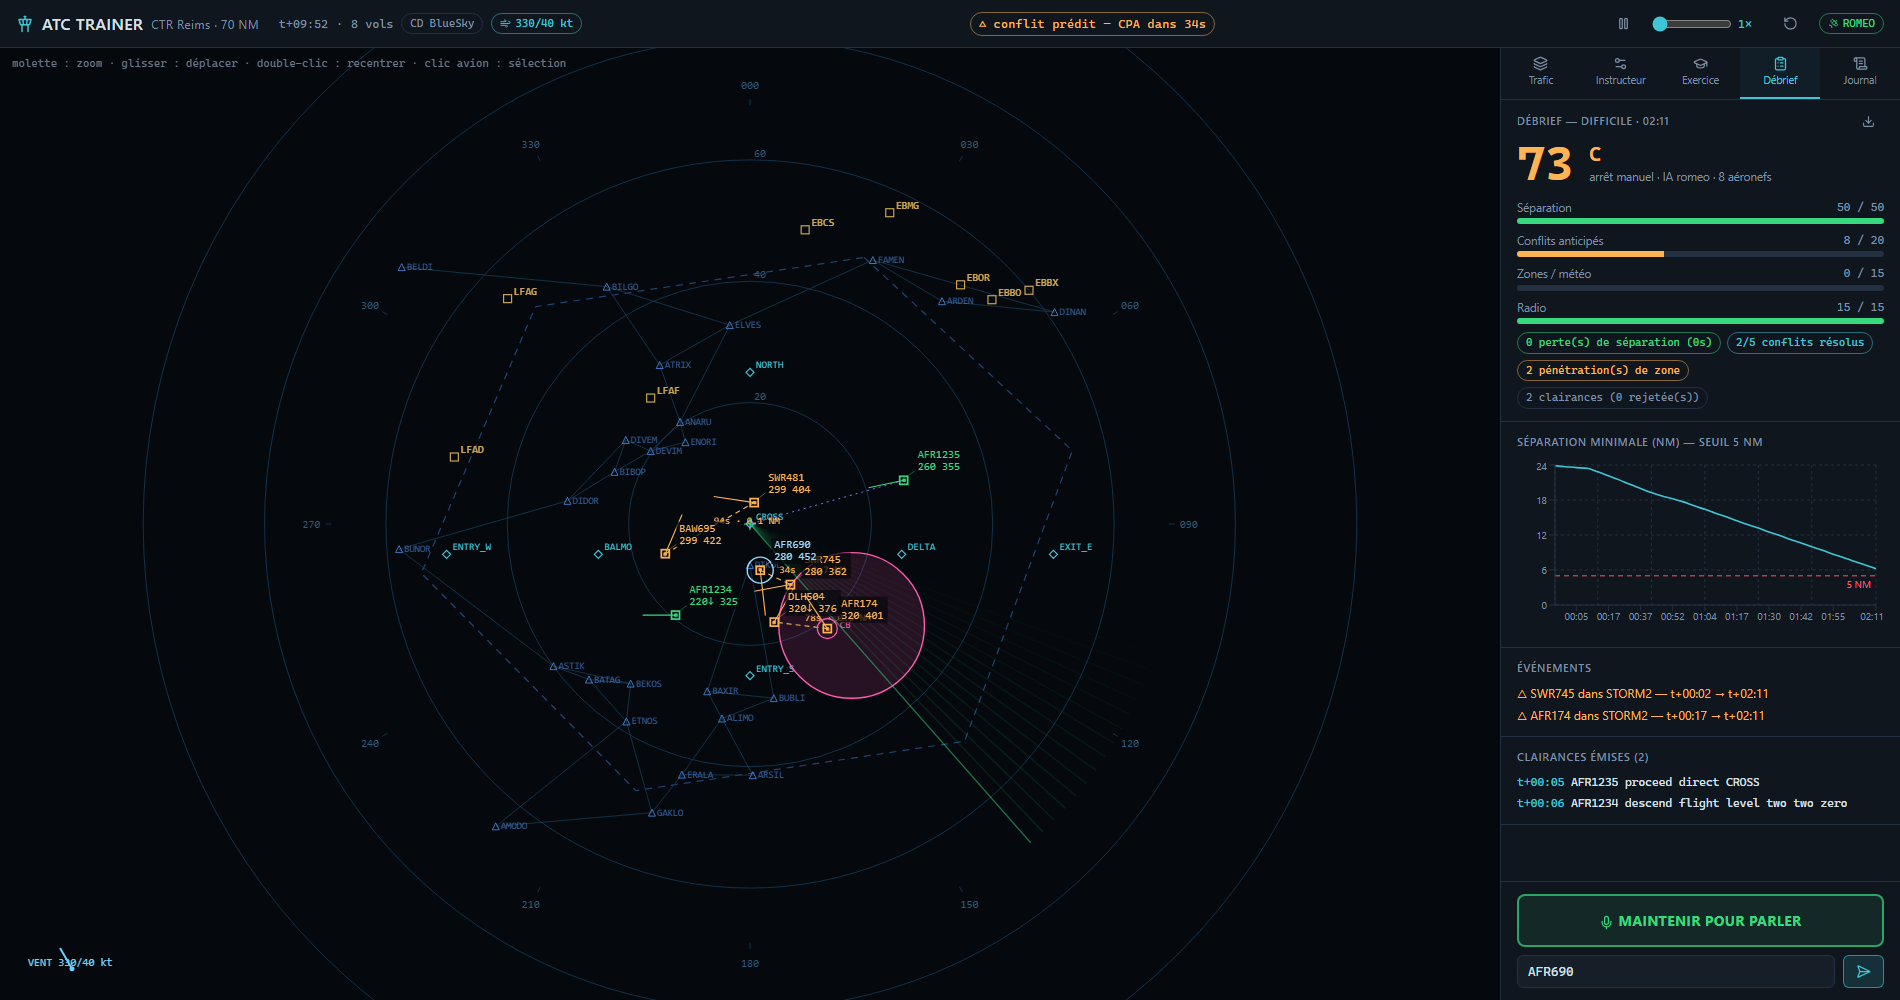
\includegraphics[width=0.82\linewidth, height=0.58\textheight, keepaspectratio]{figures/app_debrief.png}
\end{frame}

\begin{frame}{Réserve : la boucle vocale sur le cluster ROMEO}
\centering
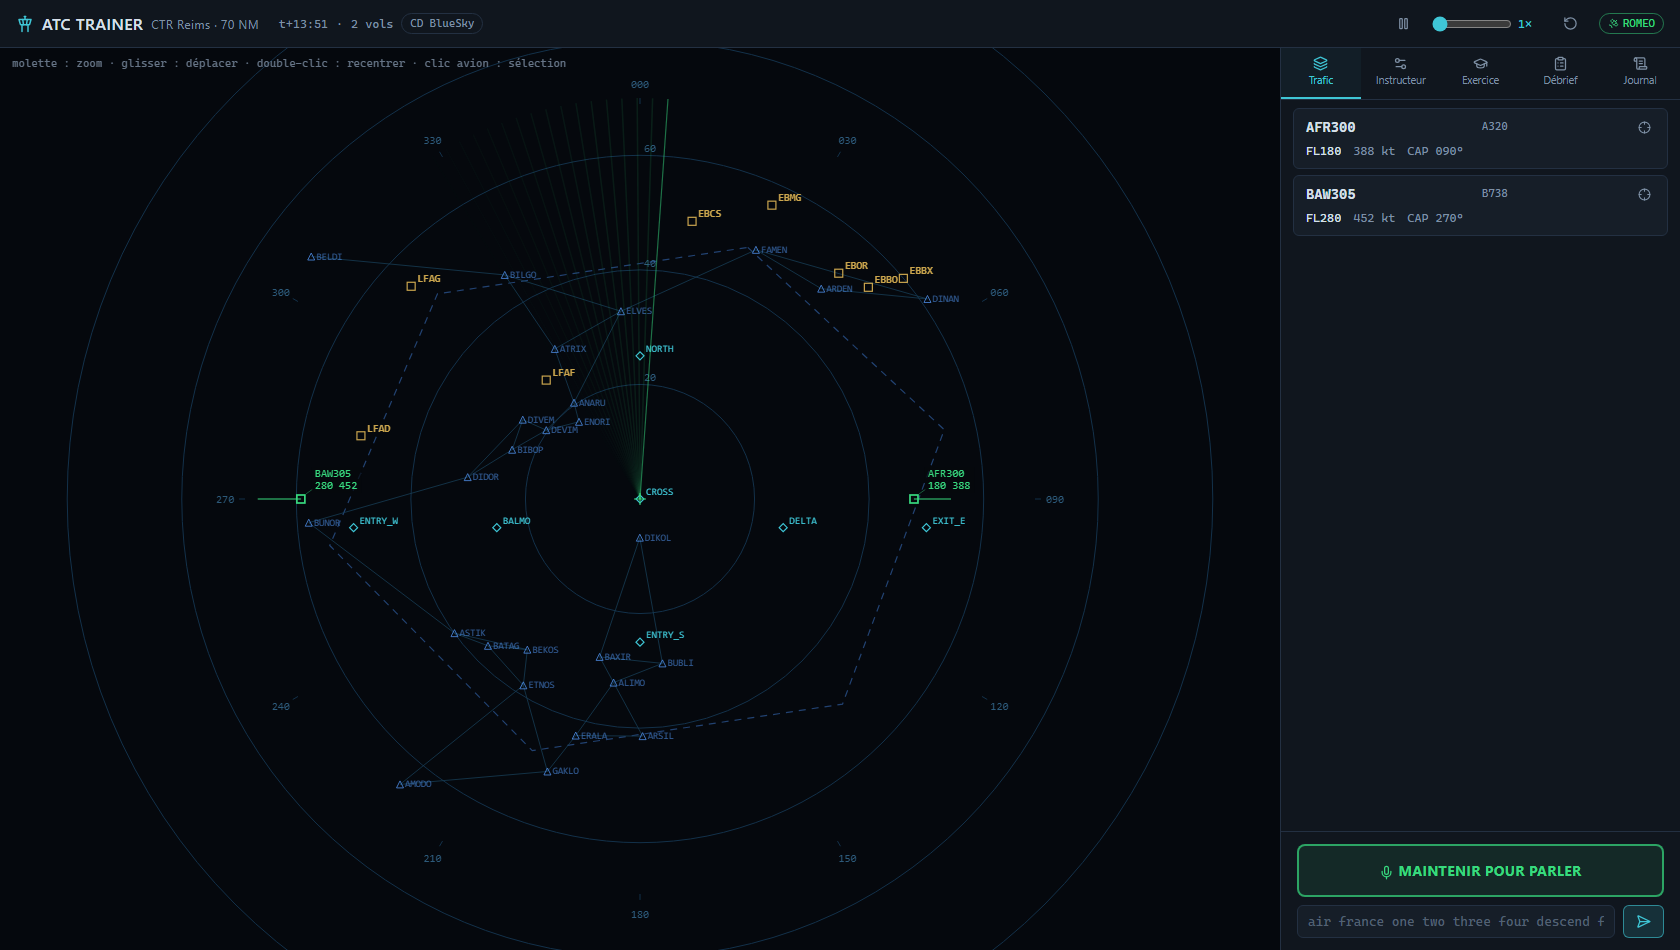
\includegraphics[width=0.80\linewidth, height=0.58\textheight, keepaspectratio]{figures/app_romeo.png}

\vspace{2pt}
{\footnotesize Semaine 8 : après une clairance parlée, AFR300 est établi au
 FL180 et collationne dans sa voix clonée.}
\end{frame}

\end{document}
